%% Hlavní soubor. Zde se definují základní parametry a odkazuje se na ostatní části. %%%

%% Verze pro jednostranný tisk:
% Okraje: levý 40mm, pravý 25mm, horní a dolní 25mm
% (ale pozor, LaTeX si sám přidává 1in)
\documentclass[12pt,a4paper]{report}
\setlength\textwidth{145mm}
\setlength\textheight{247mm}
\setlength\oddsidemargin{15mm}
\setlength\evensidemargin{15mm}
\setlength\topmargin{0mm}
\setlength\headsep{0mm}
\setlength\headheight{0mm}
% \openright zařídí, aby následující text začínal na pravé straně knihy
\let\openright=\clearpage

%% Pokud tiskneme oboustranně:
% \documentclass[12pt,a4paper,twoside,openright]{report}
% \setlength\textwidth{145mm}
% \setlength\textheight{247mm}
% \setlength\oddsidemargin{15mm}
% \setlength\evensidemargin{0mm}
% \setlength\topmargin{0mm}
% \setlength\headsep{0mm}
% \setlength\headheight{0mm}
% \let\openright=\cleardoublepage

%% Pokud používáte csLaTeX (doporučeno):
\usepackage{czech}
%% Pokud nikoliv:
%\usepackage[czech]{babel}
%\usepackage[T1]{fontenc}

%% Použité kódování znaků: obvykle latin2, cp1250 nebo utf8:
\usepackage[utf8]{inputenc}

%% Ostatní balíčky
\usepackage{graphicx}
\usepackage{amsthm}
\usepackage{amsmath}
\usepackage{listings}
\usepackage{tikz}
\usepackage{caption}
\usepackage{float}

%% Balíček hyperref, kterým jdou vyrábět klikací odkazy v PDF,
%% ale hlavně ho používáme k uložení metadat do PDF (včetně obsahu).
%% POZOR, nezapomeňte vyplnit jméno práce a autora.
\usepackage[ps2pdf,unicode]{hyperref}   % Musí být za všemi ostatními balíčky
\hypersetup{pdftitle=Nástroj pro porovnávání a vyhodnocování strojových překladů}
\hypersetup{pdfauthor=Ondřej Klejch}

%%% Drobné úpravy stylu

% Tato makra přesvědčují mírně ošklivým trikem LaTeX, aby hlavičky kapitol
% sázel příčetněji a nevynechával nad nimi spoustu místa. Směle ignorujte.
\makeatletter
\def\@makechapterhead#1{
  {\parindent \z@ \raggedright \normalfont
   \Huge\bfseries \thechapter. #1
   \par\nobreak
   \vskip 20\p@
}}
\def\@makeschapterhead#1{
  {\parindent \z@ \raggedright \normalfont
   \Huge\bfseries #1
   \par\nobreak
   \vskip 20\p@
}}
\makeatother

% Toto makro definuje kapitolu, která není očíslovaná, ale je uvedena v obsahu.
\def\chapwithtoc#1{
\chapter*{#1}
\addcontentsline{toc}{chapter}{#1}
}

\begin{document}

% Trochu volnější nastavení dělení slov, než je default.
\lefthyphenmin=2
\righthyphenmin=2

%%% Titulní strana práce

\pagestyle{empty}
\begin{center}

\large

Univerzita Karlova v~Praze

\medskip

Matematicko-fyzikální fakulta

\vfill

{\bf\Large BAKALÁŘSKÁ PRÁCE}

\vfill

\centerline{\mbox{
\includegraphics[width=60mm]{img/logo.eps}}}

\vfill
\vspace{5mm}

{\LARGE Ondřej Klejch}

\vspace{15mm}

% Název práce přesně podle zadání
{\LARGE\bfseries Nástroj pro porovnávání a vyhodnocování strojového překladu}

\vfill

% Název katedry nebo ústavu, kde byla práce oficiálně zadána
% (dle Organizační struktury MFF UK)
Ústav formální a aplikované lingvistiky

\vfill

\begin{tabular}{rl}

Vedoucí bakalářské práce: & Mgr. Martin Popel \\
\noalign{\vspace{2mm}}
Studijní program: & Informatika  \\
\noalign{\vspace{2mm}}
Studijní obor: & Obecná informatika \\
\end{tabular}

\vfill

% Zde doplňte rok
Praha 2013

\end{center}

\newpage

%%% Následuje vevázaný list -- kopie podepsaného "Zadání bakalářské práce".
%%% Toto zadání NENÍ součástí elektronické verze práce, nescanovat.

%%% Na tomto místě mohou být napsána případná poděkování (vedoucímu práce,
%%% konzultantovi, tomu, kdo zapůjčil software, literaturu apod.)

\openright

\noindent
Poděkování.

\newpage

%%% Strana s čestným prohlášením k bakalářské práci

\vglue 0pt plus 1fill

\noindent
Prohlašuji, že jsem tuto bakalářskou práci vypracoval(a) samostatně a výhradně
s~použitím citovaných pramenů, literatury a dalších odborných zdrojů.

\medskip\noindent
Beru na~vědomí, že se na moji práci vztahují práva a povinnosti vyplývající
ze zákona č. 121/2000 Sb., autorského zákona v~platném znění, zejména skutečnost,
že Univerzita Karlova v~Praze má právo na~uzavření licenční smlouvy o~užití této
práce jako školního díla podle §60 odst. 1 autorského zákona.

\vspace{10mm}

\hbox{\hbox to 0.5\hsize{%
V~........ dne ............
\hss}\hbox to 0.5\hsize{%
Podpis autora
\hss}}

\vspace{20mm}
\newpage

%%% Povinná informační strana bakalářské práce

\vbox to 0.5\vsize{
\setlength\parindent{0mm}
\setlength\parskip{5mm}

Název práce:
Nástroj pro porovnávání a vyhodnocování strojových překladů
% přesně dle zadání

Autor:
Ondřej Klejch

Katedra:
Ústav formální a aplikované lingvistiky

% dle Organizační struktury MFF UK

Vedoucí bakalářské práce:
Mgr. Martin Popel
% dle Organizační struktury MFF UK, případně plný název pracoviště mimo MFF UK

Abstrakt:
Tato bakalářská práce se zabývá vývojem nástroje pro porovnávání a vyhodnocování strojových překladů nazvaného MT-ComparEval.
V~tomto nástroji je možné porovnávat překlady na základě několika kritérií.
Mezi ně patří porovnání podle metrik strojových překladů počítaných pro celé dokumenty nebo jednotlivé věty,
  porovnání kvality překladů jednotlivých vět pomocí zvýraznění potvrzených, zlepšujících nebo zhoršujících \mbox{n-gramů}
  nebo podle souhrnu nejvíce zlepšujících či zhoršujících \mbox{n-gramů} v~celém dokumentu.
Při porovnávání dvou různých překladů nástroj MT-ComparEval také vykresluje graf s~absolutními rozdíly metrik počítaných pro jednotlivé věty a
  graf s~hodnotami z~párového bootstrap resamplingu.

Klíčová slova:
porovnání strojových překladů, vyhodnocování strojových překladačů, metriky strojových překladů
% 3 až 5 klíčových slov

\vss}\nobreak\vbox to 0.49\vsize{
\setlength\parindent{0mm}
\setlength\parskip{5mm}

Title:
Tool for Machine Translation Comparison and Evaluation
% přesný překlad názvu práce v angličtině

Author:
Ondřej Klejch

Department:
Institute of Formal and Applied Linguistics
% dle Organizační struktury MFF UK v angličtině

Supervisor:
Mgr. Martin Popel
% dle Organizační struktury MFF UK, případně plný název pracoviště
% mimo MFF UK v angličtině

Abstract:
This bachelor thesis is about development of a tool for machine translation comparison and evaluation called MT-ComparEval.
This tool allows organization of translations into groups to evaluate these against various reference translations.
With this tool it is possible to compare translations according to several criteria,
  such as evaluation by metrics of machine translations computed on whole documents or single sentences,
  quality comparison of single sentence translation with highlighting confirmed,
  improving or worsening \mbox{n-grams} or summaries of most improving or worsening \mbox{n-grams} for whole document.
MT-ComparEval can be extended by adding new machine translation metrics.


Keywords:
machine translations comparison, machine translations evaluation, machine translations metrics

\vss}

\newpage

%%% Strana s automaticky generovaným obsahem bakalářské práce. U matematických
%%% prací je přípustné, aby seznam tabulek a zkratek, existují-li, byl umístěn
%%% na začátku práce, místo na jejím konci.

\openright
\pagestyle{plain}
\setcounter{page}{1}
\tableofcontents

%%% Jednotlivé kapitoly práce jsou pro přehlednost uloženy v samostatných souborech
\chapwithtoc{Úvod}
Současný vývoj softwarových projektů probíhá v~krátkých iteracích,
  aby mohl pružně reagovat na změny v~zadání.
Stejně tak i vývoj strojových překladačů probíhá v~krátkých iteracích,
  aby bylo možné pravidelně ověřovat zlepšení nebo zhoršení kvality překladů.
Z~toho plyne potřeba vývojářů testovat změny,
  které provedli v~rámci iterace,
  která mohla trvat 30 sekund, hodinu, den nebo týden.
K~testování funkčnosti softwarových projektů lze použít různé sady testů -- od unit testů po akceptační testy.
Je možné stejným způsobem testovat i kvalitu strojových překladačů?

Je samozřejmé, 
  že vývojáři strojových překladačů testují svůj kód stejně jako ostatní vývojáři.
Pomocí těchto testů mohou zajistit,
  aby překladač fungoval,
  ale nemohou takto jednoduše zajistit kontrolu kvality překladů.
Kontrolu překladů může provádět sám vývojář,
  ale ztratí tím spoustu času a energie,
  kterou by mohl lépe využít při dalším vývoji.

Žádná kontrola kvality, kterou není možné automatizovat,
  vývojářům nepomůže zrychlit vývojový cyklus.
Proto je třeba,
  aby existoval způsob jak rychle a opakovaně kontrolovat kvalitu překladů.

Proto byly vynalezeny metriky strojového překladu,
  které umožňují rychle a opakovaně testovat překlady.
Tyto metriky se snaží hodnotit překlady tak,
  aby jejich výsledky co nejvíce odpovídaly lidskému hodnocení.

Avšak výsledek většiny metrik je pouhé jedno číslo.
Je třeba, aby vývojaři měli k~dispozici nástroje,
  pomocí kterých budou moci efektivně vyhodnocovat své překlady.
Pomocí takovýchto nástrojů si vývojáři mohou vyhodnotit,
  co způsobily změny, které provedli.

Vývojář by měl mít možnost překlady nejen vyhodnocovat,
  ale i porovnávat.
Porovnání dvou různých překladů může totiž vývojáři objasnit jevy,
  o~kterých nemusel vůbec vědět.
A~na základě takto získaných poznatků pak může vyvinout novou lepší verzi překladače.
A~po mnoha iteracích vývoje snad vyvine překladač,
  s~kterým bude moci být spokojený.

Na trhu existuje několik nástrojů,
  které umožňují vyhodnocovat překlady pomocí různých metrik
  nebo porovnávat překlady na základě různých kritérií.
Důležité je,
  aby mohl vývojář použít přístup,
  který mu vyhovuje.

Nástrojem,
  který umožňuje vývojářům efektivně porovnávat a vyhodnocovat překlady,
  se snaží být \mbox{MT-ComparEval}, 
  o~němž pojednává tato bakalářská práce.

\chapter{Motivace}
\label{chap:motivation}
V~této kapitole budou v~krátkosti představeny všechny důvody,
  proč a jak byl vyvinut nástroj \mbox{MT-ComparEval}.
Zvolená řešení pak budou více rozebrána v~následujících kapitolách.

\section{Experimenty a tasky}
Strojové překlady jsou při automatickém vyhodnocování porovnávány s~referenčním překladem
  (dále jen reference).
Vyhodnocování strojových překladačů může být zaměřeno na různé domény textu (např. novinové články, beletrie apod.) různých délek
  nebo na různé jazykové páry (např. z~angličtiny do češtiny, z~němčiny do češtiny apod.).
Aby uživatelé nástroje \mbox{MT-ComparEval} mohli snadno vyhodnocovat své strojové překladače na různých doménách nebo pro různé jazykové páry,
  mohou si vytvořit různé \textbf{\uv{experimenty}},
  v~rámci kterých mohou porovnávat své překlady s~příslušnými referencemi.
Obrázek \ref{img:experiments} ukazuje příklad vytvořených experimentů z~různých domén a jazykových párů.
\begin{figure}
	\center
	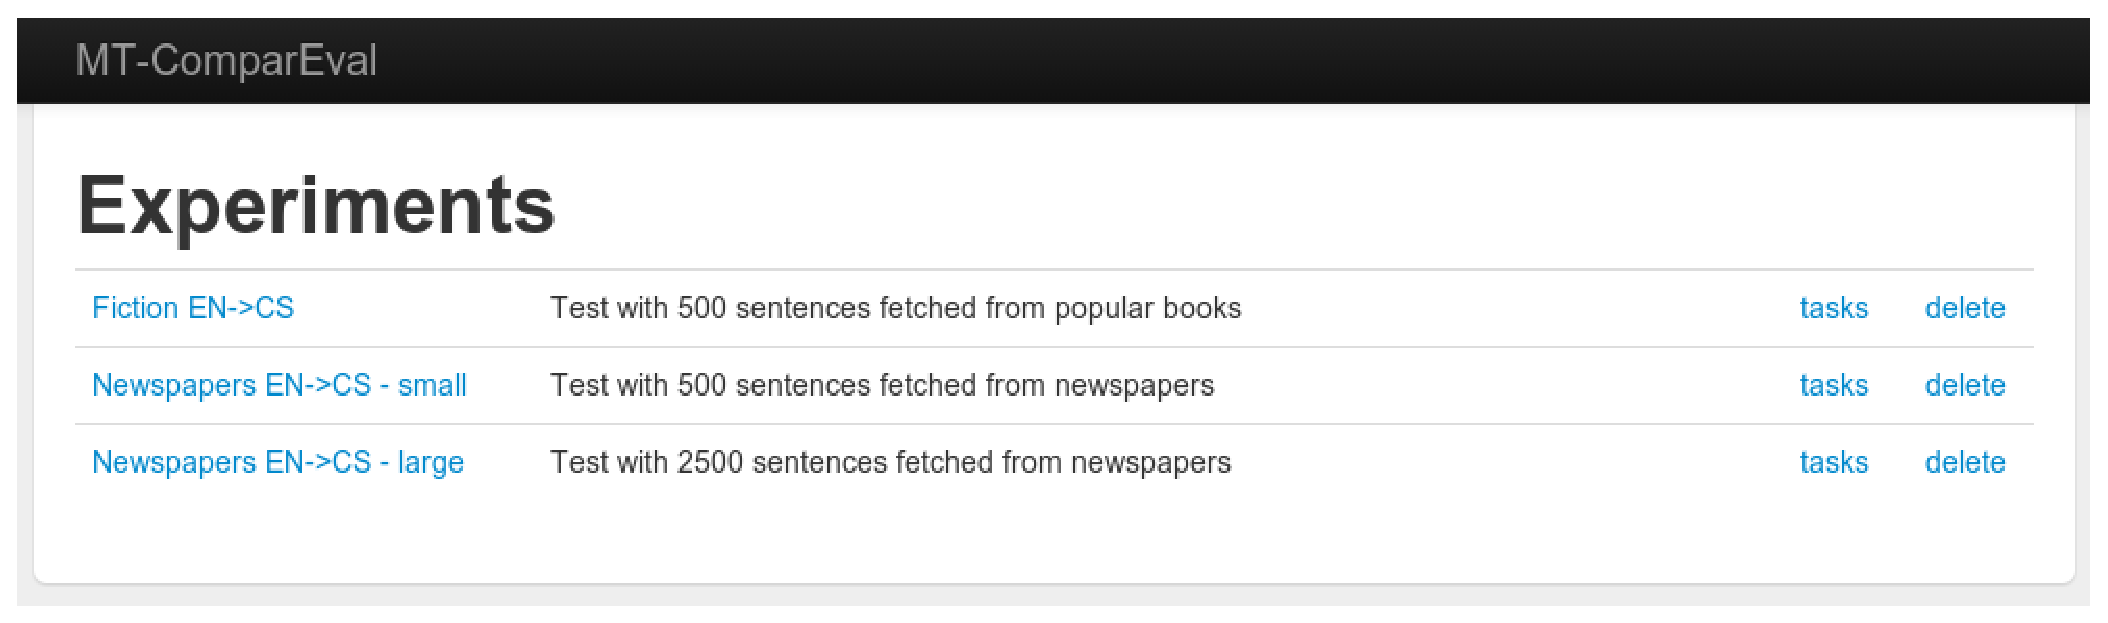
\includegraphics[width=0.9\textwidth]{img/experiments.eps}

	\caption{Přehled vytvořených experimentů v~nástroji \mbox{MT-ComparEval}}
	\label{img:experiments}
\end{figure}

V~každém experimentu pak uživatel může vytvářet \textbf{\uv{tasky}},
  které později může vyhodnocovat a porovnávat (viz Obrázek \ref{img:tasks}).
\begin{figure}
	\caption{Přehled vytvořených tasků v~jednom z~experimentů v~nástroji \mbox{MT-ComparEval}}
	\label{img:tasks}
\end{figure}

Experimenty, tasky a jiné pojmy podrobněji rozebírá ~\ref{chap:experiments}.~kapitola.


\section{Metriky strojového překladu}
K~porovnávání překladů mohou být použity metriky strojového překladu.
V~nástroji \mbox{MT-ComparEval} jsou metriky počítány na úrovni celých tasků 
  (viz Obrázek \ref{img:compare_metrics_tasks})
  i na úrovni jednotlivých vět
  (viz Obrázek \ref{img:compare_metrics_sentences}).

Metriky vypočtené na úrovni jednotlivých vět slouží i k~řazení vět ve webovém rozhraní.
Věty jsou řazeny podle absolutního rozdílu hodnoty dané metriky u~jednotlivých překladů.
Čím vyšší je tento rozdíl, tím došlo k~většímu zlepšení při~překladu dané věty.
Proto lze věty řadit podle míry zlepšení, ke které došlo během překladu dané věty. 

Z~vypočítaných metrik lze vytvořit grafy,
  které lépe ilustrují rozdíl v~kvalitě jednotlivých překladů.
Nástroj \mbox{MT-ComparEval} obsahuje graf rozložení absolutního rozdílu výsledků metrik v~jednotlivých větách (viz Obrázek \ref{img:chart-metrics-sentences})
  a graf zobrazující rozdíly metrik celých dokumentů získaných pomocí párového bootstrap resamplingu (viz Obrázek \ref{img:chart-metrics-bs}).

Metrikami strojových překladů se více zabývá \ref{chap:metrics}. kapitola.
V~té budou představeny všechny metriky,
  které jsou použity v~nástroji \mbox{MT-ComparEval}.


\begin{figure}
	\caption{Porovnání metrik dvou tasků v~nástroji \mbox{MT-ComparEval}.}
	\label{img:compare_metrics_tasks}
\end{figure}

\begin{figure}
	\caption{Porovnání metrik dvou překladů v~nástroji \mbox{MT-ComparEval}.}
	\label{img:compare_metrics_sentences}
\end{figure}

\begin{figure}
	\caption{Graf zobrazující rozdělení absolutních rozdílů metrik spočtených na jednotlivých větách.}
	\label{img:chart-metrics-sentences}
\end{figure}

\begin{figure}
	\caption{Graf zobrazující rozdíly metrik získaných pomocí párového bootstrap resamplingu.}
	\label{img:chart-metrics-bs}
\end{figure}

\section{Porovnávání dvou strojových překladů}
Kvalitu strojových překladačů je možné vyhodnotit i porovnáním jednotlivých vět.
Nástroj \mbox{MT-ComparEval} umožňuje procházet věty seřazené podle metriky strojových překladů 
  a hledat v~těchto větách rozdíly,
  které ovlivnily výsledné metriky.
Aby uživatelé mohli snadněji vyhledat rozdíly mezi větami,
  je možné zobrazit potvrzené \mbox{n-gramy} (\mbox{n-gramy}, které se nachází v~referenci i strojovém překladu),
  zlepšující \mbox{n-gramy} (potvrzené \mbox{n-gramy}, které se nachází pouze v~jednom z~porovnávaných překladů)
  nebo zhoršující \mbox{n-gramy} (nepotvrzené \mbox{n-gramy}, které se nachází pouze v~jednom z~porovnávaných překladů).
Na Obrázku \ref{img:compare_sentences} je vidět porovnání dvou překladů se zvýrazněnými \mbox{n-gramy}.

Strojové překlady nemusí být porovnávány pouze na základě strojových metrik,
  další informací,
  díky které je možné si vytvořit lepší představu o~vlastnostech strojového překladače,
  jsou přehledy nejvíce zlepšujících a zhoršujících \mbox{n-gramů} v~jednotlivých překladech (viz Obrázek \ref{img:confirmed_ngrams}).

Přehledy zlepšujících i zhoršujících \mbox{n-gramů} mohou být použity k~filtrování vět,
  aby si uživatel mohl snadno prohlédnout věty,
  ve kterých se dané \mbox{n-gramy} nachází.
Na Obrázku \ref{img:filtered_sentences} je vidět výpis vět obsahujících zlepšující \mbox{n-gram} ??.

\begin{figure}
	\caption{
		Porovnání dvou překladů v~nástroji \mbox{MT-ComparEval}.
		Pastelovými odstíny žluté a modré barvy jsou zvýrazněny potvrzené \mbox{n-gramy},
		sytými odstíny žluté a modré barvy jsou zvýrazněny zlepšující \mbox{n-gramy}
		a červenou barvou jsou zvýrazněny zhoršující \mbox{n-gramy}.
	}
	\label{img:compare_sentences}
\end{figure}

\begin{figure}
	\caption{Přehled nejvíce zlepšujících \mbox{n-gramů} v~jednotlivých překladech.}
	\label{img:confirmed_ngrams}
\end{figure}

\begin{figure}
	\caption{Výpis vět, ve kterých se nachází zlepšující \mbox{n-gram} ??}
	\label{img:filtered_sentences}
\end{figure}

O~algoritmech,
  které byly použity při porovnávání dvou překladů,
  a hledání pozic potvrzených \mbox{n-gramů}
  pojednává \ref{chap:compare}. kapitola.


\section{Automatizace a snadné použití}
Nástroj \mbox{MT-ComparEval} byl navržen tak,
  aby bylo možné jeho použití co nejvíce automatizovat.
Uživatelé proto nemusí ručně vytvářet každý task,
  ale mohou si napsat jednoduché skripty,
  pomocí nichž mohou vytvářet tasky v~nástroji \mbox{MT-ComparEval} automaticky při každé změně strojového překladače.

V~\ref{chap:users}. kapitole je možné najít informace,
  jak se používá nástroj \mbox{MT-ComparEval}
  a jak je možné nasadit ho do vývojového procesu.

\section{Rozšiřitelnost}
Nástroj \mbox{MT-ComparEval} si neklade za cíl implementovat co nejvíce metrik,
  proto jsou v~něm předprogramovány pouze některé.
Zároveň je však umožněno doprogramovat si vlastní metriky.

O~tom, jak si uživatel může doprogramovat vlastní metriky nebo jak byl nástroj \mbox{MT-ComparEval} vyvinut,
  je možné se dočíst v~\ref{chap:programmers}. kapitole.


\chapter{Názvosloví MT-ComparEval}
\label{chap:experiments}

Správné pochopení pojmů \textbf{experiment},\textbf{task}, \textbf{\mbox{n-gram}}, \dots je důležité k pochopení fungování celého nástroje MT-ComparEval.
Proto v této kapitole bude podrobněji vysvětleno,
  co tyto pojmy znamenají a jaké jsou mezi nimi vztahy.

\section{Experiment}
Uživatelé mohou chtít testovat své překladače na různých textových doménách různých délek
  nebo testovat své překladače pro různé jazykové páry.
Nástroj MT-ComparEval musí umožňovat vytvořit různá vyhodnocovací prostředí,
  ve kterých uživatelé mohou testovat své strojové překladače.
Takovéto testovací prostředí se v nástroji MT-ComparEval nazývá \textbf{experiment}.

Každý experiment obsahuje vlastní \textbf{zdroj} (věty, které mají být strojovým překladačem přeloženy) a
  \textbf{referenci} (člověkem přeložené věty, které budou později použity k vyhodnocování jednotlivých strojových překladačů).
Pomocí různých dvojic zdrojů a referencí mohou uživatelé vyhodnocovat strojové překladače na různých testovacích sadách,
  což se jim může hodit v případě,
  kdy se překladač na různých zdrojích chová různě.

\section{Task}
V rámci experimetu uživatelé mohou chtít porovnávat různé překlady zdrojových vět.
Ať už se jedná o různé verze jednoho strojového překladače nebo různé strojové překladače.
Aby mohl uživatel vyhodnocovat různé překlady,
  umožňuje nástroj MT-ComparEval nahrávat do experimentů tzv. \textbf{tasky}.
Každý task reprezentuje jednu verzi překladu zdrojových vět,
  která později může být porovnána s jinou verzí překladu.
V rámci této bakalářské práce budou strojové překlady nazývány zkráceně slovem \textbf{překlady}.

O vytváření experimentů a tasků i o dalších možnostech použití nástroje MT-ComparEval je možné se dozvědět v \ref{chap:users}. kapitole.

\section{N-gramy}
Při vysvětlování počítání strojových metrik
  nebo popisu, jak jsou porovnávány dva překlady jedné věty,
  jsou často použity termíny spojené se slovem \mbox{n-gram}.
Proto budou všechny tyto termíny v této části vysvětleny,
  aby pozdější výklad byl jasný a nemuselo se odbíhat od tématu.

Posloupnost n po sobě jdoucích slov\footnote{
  Často se používá i výraz \textbf{token}. Token může být jak slovo, tak interpunkční znaménko a do \mbox{n-gramů} mohou patřit i interpunkční znaménka}
  se nazývá \textbf{\mbox{n-gram}}.
N-gramy,
  které se nacházejí i v referenci i ve strojovém překladu,
  se v rámci nástroje MT-ComparEval nazývají \textbf{potvrzené \mbox{n-gramy}}.
Potvrzené \mbox{n-gramy},
  které se při porovnávání dvou překladů nacházejí pouze v jednom z nich,
  jsou nazývány \textbf{zlepšující \mbox{n-gramy}}.
N-gramy,
  které nejsou potvrzené referencí
  a při porovnávání dvou překladů se nacházejí pouze v jednom z nich,
  jsou nazývany \textbf{zhoršující \mbox{n-gramy}}.
O významu jednotlivých typů \mbox{n-gramů} je možné si udělat lepší představu na Obrázku \ref{img:n-grams}.

\begin{figure}

	\caption{
		Porovnání dvou překladů v nástroji MT-ComparEval.
		Pastelovými odstíny žluté a modré barvy jsou zvýrazněny potvrzené \mbox{n-gramy},
		sytými odstíny žluté a modré barvy jsou zvýrazněny zlepšující \mbox{n-gramy}
		a červenou barvou jsou zvýrazněny zhoršující \mbox{n-gramy}.
	}
	\label{img:n-grams}
\end{figure}


\chapter{Metriky strojového překladu}
\label{chap:metrics}

Při porovnávání dvou strojových překladů je potřeba,
  abychom byli schopní snadno a rychle určit,
  jak jsou jednotlivé překlady dobré.
Posuzování kvality překladů člověkem je časově náročné
  a není možné ho automatizovat.
Proto byly vytvořeny metriky,
  jejichž výsledky jsou podobné výsledkům získaných od lidí,
  ale je možné je rychle spočítat,
  aplikovat na různé jazyky a opakovat dle libosti.
Mezi tyto metriky patří i metrika BLEU,
  která je zvolena jako výchozí metrika v~nástroji MT-ComparEval.

Při počítání metrik strojových překladů se snažíme zjistit,
  jak moc se strojový překlad podobá překladu od člověka -- tzv. referenčnímu překladu.
Čím více se podobá strojový překlad překladu referenčnímu,
  tím je lepší.
To ovšem neznamená, že překlad s~nižší hodnotou metriky je špatný.
Překlad totiž můžeme provést několika různými způsoby 
  ( např. můžeme změnit slovosled, použít synonyma, \dots ),
  z~nichž se pouze jeden bude shodovat s~referenčním překladem.
Tento problém může zmírnit použití více referenčních překladů,
  ale úplně odstranit ho nelze.
Některé překladatelské systémy jsou optimalizovány pro určité metriky,
  avšak jejich výsledný překlad nemusí být ideální.
Proto je třeba,
  abychom při vyhodnocování strojového překladu nespoléhali pouze na jednu metriku.


\section{BLEU}
Nejvíce používanou metrikou pro vyhodnocování překladů je metrika BLEU.
Hlavním důvodem je to,
  že hodně odpovídá lidskému vyhodnocení překladu
  a je možné ji rychle spočítat.
Rychlost výpočtu metrik je pro vývojáře překladových systémů velmi důležitá,
  protože vývojáři potřebují každou změnu v~systému otestovat,
  aby si mohli být jisti,
  že překladový systém nepokazili.

Při počítání metriky BLEU počítáme precision \mbox{n-gramů},
  což nám říká,
  kolik \mbox{n-gramů} z~vyhodnocovaného překladu se nachází i v~referenčním překladu.	
$$ \text{PRECISION} = \frac{\lvert \lbrace \text{\mbox{n-gramy} z~referenčního překladu} \rbrace \cap \lbrace \text{\mbox{n-gramy} z~vyhodnocovaného překladu} \rbrace \rvert}{\lvert \lbrace \text{\mbox{n-gramy} z~vyhodnocovaného překladu} \rbrace \rvert}$$

Pří hledání potvrzených \mbox{n-gramů} si musíme dát pozor na překlady,
  ve kterých se nachází více stejných \mbox{n-gramů} než je daných \mbox{n-gramů} v~referenčním překladu.
V~takovém případě vezmeme vždy jen
  $min( \lvert \lbrace \text{\mbox{n-gramy} z~referenčního překladu} \rbrace \cap \lbrace \text{\mbox{n-gramy} z~vyhodnocovaného překladu} \rbrace \rvert, \lvert \lbrace \text{\mbox{n-gramy} z~referenčního překladu} \rbrace \rvert )$
V~článku o~BLEU pomocí takto nalezených potvrzených \mbox{n-gramů} počítají modified \mbox{n-gram} precision:
$$ \text{MODIFIED PRECISION} = \frac{ \lvert \text{potvrzené \mbox{n-gramy}} \rvert }{ \lvert \text{\mbox{n-gramy} z~vyhodnocovaného překladu} \rvert } $$




\section{BLEUS}
Abychom mohli počítat metriku BLEU i pro jedntolivé věty,
  musíme se vypořádat s~tím,
  že se v~některých větách nemusí vyskytovat žádné potvrzené 1-gramy, 2-gramy, 3-gramy nebo 4-gramy.
V~tom případě by výsledná metrika těchto vět byla rovna nule,
  i když by se v~nich nějaký potvrzený \mbox{n-gram} nacházel.
Tento problém řeší vylepšení metriky BLEU -- metrika BLEUS. %% přidat citaci
Ta připočítává +1 ke všem \mbox{n-gramům} delším než jedna.
Tím pádem můžeme spočítat metriku i pro věty,
  které nemají potvrzené \mbox{n-gramy} libovolné délky.
Zároveň dokážeme ohodnotit úplně špatný překlad nulovou metrikou,
  protože 1-gramy vyhlazovány nejsou.

Skript mteval-13a.pl, %% přidat citaci
  který je ve světě považován za autoritu pro vyhodnocování překladů,
  používá jiný způsob vyhlazování.
Místo přičítání +1 ke všem \mbox{n-gramům} má speciální vzoreček pro počítání precision o~chybějících potvrzených \mbox{n-gramů}.
Precision je rovna $1 / 2^k$, kde $k = 1$ u~první n takové,
  že v~překladu není žádný potvrzený \mbox{n-gram}.

Rozdíl obou metrik si můžeme demonstrovat na větě délky 4,
  která obsahuje pouze jeden potvrzený 2-gram
  (z~čehož plyne, že obsahuje i dva potvrzené 1-gramy).

\begin{tabular}{| l | c | c || c | c |}
\hline
& & & \multicolumn{2}{c|}{PRECISION} \\
\cline{4-5}
délka & počet potvrzených & celkový počet & BLEUS & mteval \\
\hline
1-gram & 2 & 4 & $\frac{2}{4} = 0.50$ & $\frac{2}{4} = 0.50$ \\
2-gram & 1 & 3 & $\frac{1+1}{3+1} = 0.50$ & $\frac{1}{3} \approx 0.33$ \\
3-gram & 0 & 2 & $\frac{0+1}{2+1} \approx 0.33$ & $\frac{1}{2^1} = 0.50$ \\
4-gram & 0 & 1 & $\frac{0+1}{1+1} = 0.50$ & $\frac{1}{2^2} = 0.25$ \\
\hline \hline 
\multicolumn{3}{ |r| }{bleu} & $\frac{1}{2^3 3}$ & $\frac{1}{2^4 3}$ \\
\hline
\end{tabular}

To, že se metriky liší,
  nám vůbec nevadí,
  protože obě metriky ve většině případů dokáží rozpoznat lepší překlad od horšího.

Problém, se kterým se vyhlazování u~obou přístupů nedokáže vypořádat, je,
  když porovnáváme dva překlady, z~nichž jeden je kratší než 4 slova. 
Vyhlazovaní u~mteval používá výjimku u~precision \mbox{n-gramů},
  kde n je větší než počet slov ve větě. 
U~těchto \mbox{n-gramů} nastavuje precision rovno jedné.
Krátší překlad, který může být horší,
  pak bude vyhodnocen jako lepší než skutečně lepší překlad.

Chybu si můžeme ukázat na dvou větách.
První věta dlouhá dvě slova nebude obsahovat žádné potvrzené \mbox{n-gramy}.

\begin{tabular}{| l | c | c || c | c |}
\hline
& & & \multicolumn{2}{c|}{PRECISION} \\
\cline{4-5}
délka & počet potvrzených & celkový počet & BLEUS & mteval \\
\hline
1-gram & 1 & 2 & $\frac{1}{2} = 0.50$ & $\frac{1}{2} = 0.50$ \\
2-gram & 0 & 1 & $\frac{0+1}{1+1} = 0.50$ & $\frac{1}{2^1} = 0.50$ \\
3-gram & 0 & 0 & $\frac{0+1}{0+1} = 1$ & 1 \\
4-gram & 0 & 0 & $\frac{0+1}{0+1} = 1$ & 1 \\
\hline \hline 
\multicolumn{3}{ |r| }{bleu} & $\frac{1}{2^2}$ & $\frac{1}{2^2}$ \\
\hline
\end{tabular}

Jako druhou použijeme větu z~předchozího příkladu,
  pro níž vyšlo vyhlazené BLEUS$ = \frac{1}{2^3 3}$
  a mteval$= \frac{1}{2^4 3}$.
U~horšího překladu tak vyšlo BLEUS $6\times$ větší a mteval $12\times$ větší. 
Díky této nemilé vlastnosti vyhlazování BLEU se může stát,
  že při procházení vět nenajdeme takto špatný překlad,
  protože bude vyhodnocen jako lepší.

\section{Potvrzené \mbox{n-gramy}}
Abychom částečně napravili chyby popsané výše,
  můžeme jako metriku zavést počet potvrzených \mbox{n-gramů} v~překladu.
Touto metrikou bude vždy horší překlad označen za horší,
  ale problém nastane při řazení podle absolutního rozdílu,
  protože v~delších větách může být více potvrzených \mbox{n-gramů},
  budou většinou dlouhé věty předcházet kratší věty,
  u~kterých se správnost překladu mohla mnohem více lišit.

\section{Recall}
Pří výpočtu BLEU se počítá precision \mbox{n-gramů} ze strojového překladu.
Pokud místo \mbox{n-gramů} ze strojového překladu použijeme \mbox{n-gramy} z~referenčního překladu,
  vyjde nám metrika Recall,
  která říká s~jakou pravděpodobností se nachazí \mbox{n-gram} z~referenčního překladu i v~překladu strojovém.
$$ RECALL = \prod_{l=1}^{4} \frac{ \lvert \text{potvrzené \mbox{n-gramy} délky l} \rvert }{ \lvert \text{referenční \mbox{n-gramy} délky l} \rvert } $$

Touto metrikou, případně s~vyhlazením stejným jako v~BLEUs,
  budeme moci vyřešit oba dva výše zmíněné problémy -- 
  t.j. problém s~krátkým překladem a problém s~řazením podle potvrzených \mbox{n-gramů}.

Nicméně i Recall má své problémy.
Strojové překlady,
  které jsou výrazně delší než překlady referenční,
  by mohly mít vysokou hodnotu Recall,
  ale i tak by se jednalo o~špatné překlady,
  protože by obsahovaly mnoho nadbytečných slov. 
Tento problém řeší metrika F-Measure,
  která bude vysvětlena v~následující části.

\section{F-Measure}
Metrika F-Measure kombinuje Recall i Precision,
  čímž zajišťuje, 
  že zbytečně dlouhé překlady budou mít horší výsledky.

$$ \text{F-MEASURE} = 2 \cdot \frac{\text{PRECISION} \cdot \text{RECALL}}{\text{PRECISION} + \text{RECALL}} $$

\section{Diskuse}

\newtheorem*{define}{Definice}	% Definice nečíslujeme, proto "*"
\newtheorem*{example}{Příklad}	% Příklady nečíslujeme, proto "*"

\chapter{Zvýrazňujeme výsledky porovnání dvou systémů}
Při vyhodnocování strojových překladů nás zajímá,
  která slova a slovní spojení byly přeloženy správně (potvrzené n-gramy)
  a které správně přeloženy nebyly (nepotvrzené n-gramy).
Při porovnávání dvou překladových systémů chceme zvýraznit slova a slovní spojení,
  které byly přeloženy:

\begin{itemize}
  \item Správně v obou porovnávaných systémech \\
    Tato slova nepřispěla k zlepšení ani k zhoršení BLEU žádného
    z porovnávaných překladových systémů.
  \item Správně v jednom z porovnáváných systémů \\
    Tato slova přispěla k zlepšení BLEU překladového systému
  \item Špatně pouze v jednom z porovnávaných systémů \\
    Tato slova přispěla k zhoršení BLEU překladového systému
\end{itemize}

\section{Hledáme pozice potvrzených n-gramů}


Nejjednodušší práci máme,
  pokud je počet výskytů jednotlivých n-gramů ve strojovém překladu
  menší nebo roven počtu výskytů odpovídajících n-gramů v referenčním překladu.
Pak můžeme všechny n-gramy,
  které mají alespoň jednu podoporu v referenčním překladu,
  zvýraznit jako n-gramy potvrzené.

Horší situace nastane,
  pokud bude počet výskytů některého n-gramu ve strojovém překladu
  vysšší než počet výskytů odpovidajících n-gramů v referenčním překladu.

\subsection{Vybíráme si z několika možností}
Při vyhodnocování strojových překladů můžeme narazit na situaci,
  kdy se ve strojovém překladu nachází více výskytů n-gramu než v referenčním překladu.
Naším úkolem tedy je, abychom zvýraznili výskyty n-gramů,
  které nejvíce odpovídají výskytům n-gramů v referenčním překladu.

\begin{example}
{\sl RT} A , B C\\
{\sl MT} A , B , C \\
\end{example}

\begin{define}
{\sl Nejdelší společná podposloupnost(LCS)} posloupností A a B, je posloupnost,
  kterou můžeme získat z posloupností A a B odstraněním některých prvků. 
\end{define}

Výskyty n-gramů, které se nacházejí v nejdelší společné podposloupnosti,
  jsou z definice LCS 

\subsection{Odhalujeme špatný slovosled}
Další problém, na který můžeme často narazit, je změna slovosledu.
S tou si metoda používající global alignment neporadí. 

\begin{example}
{\sl RT} A B C D \\
{\sl MT} A C B D \\
\end{example}

\subsection{Nevýhody tohoto řešení}


\chapter{Uživatelská dokumentace}
\label{chap:users}

\section{Systémové požadavky}
Nástroj \mbox{MT-ComparEval} byl vyvinut jako webová aplikace,
  která poběží na serveru s~Linuxem.\footnote{
    Pokud je aplikace nainstalována na vzdáleném serveru, může být používána pomocí libovolného moderního webového prohlížeče na libovolném operačním systému.
  }
Dále musí být na uživatelském počítači nainstalované PHP 5.4 a databáze SQLite 3.

\section{Instalace a spuštění programu}
Instalace není vůbec náročná,
  stačí spustit script \textbf{./bin/install.sh},
  který připraví vše potřebné pro běh programu. 
Jelikož chceme,
  aby uživatel nemusel používat webserver Apache nebo jiné webservery,
  musí si uživatel před každým spuštěním aplikace zapnout lokální server pomocí skriptu \textbf{./bin/server.sh},
  který spustí aplikaci na adrese \textbf{http://localhost:8080}.
Poslední věc,
  kterou je třeba při spouštění aplikace udělat, je,
  aby uživatel spustil program,
  který kontroluje nově přidané experimenty a tasky.
Ten se spustí pomocí skriptu \textbf{./bin/watcher.sh}.
Pro celkové zjednodušení spouštění aplikace byl přidán skript,
  který všechny tyto kroky sjednotí do jednoho,
  a proto je možné spustit celou aplikaci pomocí příkazu \textbf{./bin/run.sh}.

V~případě, že má uživatel nainstalován nějaký webový server
  a chce ho použít pro provoz nástroje \mbox{MT-ComparEval},
  může ho použít jako v~případě ostatních webových stránek,
  ale nesmí zapomenout spustit skript pro kontrolu nově přidaných experimentů a tasků.

\section{Import experimentů}
Aby uživatel mohl porovnávat překlady,
  musí nejprve vytvořit experiment,
  v~jehož rámci bude jednotlivé překlady vyhodnocovat.
Každý experiment je uložen ve vlastním podadresáři adresáře \textbf{./data},
  do kterého uživatel musí nahrát zdrojový text a referenční překlad.
Výchozí jména souborů jsou \textbf{source.txt} pro zdrojový překlad
  a \textbf{reference.txt} pro referenční překlad.
U~všech souborů s~větami se předpokladá,
  že každá věta či souvětí je na vlastním řádku
  a je zachováno pořadí vět.
To znamená, že první řádek v~souboru se zdrojovým textem je přeložen na prvním řádku souboru s~referenčním a strojovým překladem,
  druhý řádek v~souboru se zdrojovým textem odpovídá druhému řádku v souboru s referencí atd..
Pro správný běh aplikace je nutné, aby soubory se zdrojovým textem a referenčním překladem měly stejný počet řádků.
Pokud nebudou mít stejný počet řádků, experiment nebude importován.
Jako jméno experimentu je použito jméno adresáře.

\subsection{Konfigurace experimentu}
Výše zmíněný přístup je trošku omezený a nenabízí uživatelům možnosti konfigurace.
Proto je možné,
  aby si uživatel v~konfiguračním souboru \textbf{./config.neon} předefinoval výchozí hodnoty.
Je tak možné změnit jméno experimentu, popisek experimentu nebo jména souborů,
  ve kterých se bude hledat zdrojový text či referenční překlad.

Konfigurace experimentu by mohla vypadat například takto: \\

\begin{verbatim}
name: Nakonfigurovaný experiment
description: Ukázka konfigurace experimentu
source: zdrojovy_text.txt
reference: referencni_preklad.txt
\end{verbatim}

Pole name odpovídá názvu experimentu, které bude použito místo jména adresáře.
Description je jednořádkový popis experimentu,
  který odpovídá např. hlavičce commit message.
Source a reference jsou relativní jména souborů,
  ze kterých bude načten zdrojový text resp. referenční překlad.

Informace o~importu experimentu je možné nalézt
  jak v~lokálním logu každého experimentu v~souboru \textbf{./data/experiment/import.log},
  tak v~globálním logu všech importů v~souboru \textbf{./log/import.log}.
Z~toho logu uživatel může poznat,
  jestli byl daný experiment úspěšně importován,
  případně k~jakému problému při importu došlo.

V~případě, že se import nezdaří,
  může uživatel opravit chyby,
  kvůli kterým byl import přerušen,
  a znovu experiment nahrát do daného adresáře.
Musí však smazat soubor \textbf{./data/experiment/.notimported},
  který zabraňuje dalším importům u~experimentů,
  při jejichž importu došlo k~chybě.


\section{Import tasků}
Překlad,
  který cheme importovat k~porovnání v~rámci experimentu,
  v~nástroji \mbox{MT-ComparEval} nazýváme task.
Tasky nahráváme jako podadresáře v~adresáři experimentu,
  s~jehož referenčním překladem chceme daný překlad porovnat.
Jediný soubor, který musíme do tohoto podadresáře nahrát je \textbf{translation.txt},
  v~kterém budou všechny přeložené věty.
Opět je nutné, aby soubor s přeloženými větami měl stejný počet řádků jako soubor s referenčním překladem.
Jméno tasku je stejné jako jméno podadresáře.

\subsection{Konfigurace tasku}
Stejně jako je možné konfigurovat experiment je možné konfigurovat i task.
Task má konfigurovatelné jméno (name), popisek (description),
  relativní cestu k~souboru s překladem (translation) a volbu,
  zda chceme předpočítávat zlepšující a zhoršující \mbox{n-gramy} (precompute\_ngrams).
U~všech tasků, pokud uživatel neřekne jinak, 
  jsou tyto \mbox{n-gramy} předpočítány.
Konfigurace tasku může vypadat například takto:

\begin{verbatim}
name: Nakonfigurovaný task
description: Ukázka konfigurace task
translation: preklad.txt
precompute_ngrams: false
\end{verbatim}

Záznam o~průběhu importu je uložen v~adresáři tasku v~soboru \textbf{import.log},
  pomocí něhož můžeme odhalit případné problémy při importu
  a následně je odstranit stejným způsobem jako tomu bylo při importu experimentu.

V~obou konfiguračních souborech není nutné konfigurovat všechny položky.
Pokud bude některá položka vynechána,
  bude použita její výchozí hodnota. 

\section{Webové prostředí}
Porovnávání tasků je realizováno pomocí webové aplikace,
  která při zapnutém lokálním serveru běží na adrese \textbf{localhost:8080}.
Uživatel si nejprve musí zvolit experiment,
  jehož tasky chce porovnávat a následně si z~těchto tasků vybere dva k~porovnání.
%% vložit obrázek s výpisem experimentu
%% vlozit obrázek s výpisem tasku

V~případě,
  že uživatel již v~budoucnu nebude chtít používat daný experiment nebo task,
  může jej smazat pomocí příslušného odkazu ve webovém prostředí.

\subsection{Porovnávání tasků}
K~porovnání dvou tasků je možné přistoupit z~několika pohledů.
Každému pohledu odpovídá jedna záložka v~horním menu stránky s~porovnáním.
Kvalitu překladu tasku je možné posuzovat na základě překladu jednotlivých vět,
  vypočtených metrik nebo nalezených zlepšujících resp. zhoršujících \mbox{n-gramů}.
Při porovnávání si uživatel může zvolit metriku,
  podle níž se bude řídit výpis vět nebo grafů metrik.
Změnou metriky se tak mění pořadí vět,
  grafy s~rozdílem hodnot metriky na úrovni jednotlivých vět
  a grafem s~hodnotami z~párového bootstrap resamplingu.
Ve výchozím nastavení se věty zobrazují od nejvíce zlepšujících po nejvíce zhoršující,
  ale toto pořadí lze stejně jako metrika snadno změnit.\footnote{
    Míra zlepšení daného překladu je určena rozdílem aktivní metriky u porovnávaných překladů.
  }

V~případě potřeby je možné přímo v~porovnání měnit jaké tasky se mají porovnávat,
  což může být výhodné v~případě,
  že uživatele zajímá,
  jak by jeden z~porovnávaných tasků obstál v~porovnání s~jiným.
%% vložit obrázek s horní lištou

\subsubsection{Věty}
Záložka \textbf{Sentences} slouží k~zobrazení všech vět z~obou překladů.
U~každé věty se zobrazuje zdrojový text,
  referenční překlad, oba porovnávané překlady
  a metriky jednotlivých překladů.
Každou z~těchto informací je možné zobrazit/skrýt pomocí panelu \textbf{Options}.
Jak již bylo zmíněno dříve,
  věty jsou seřazeny podle rozdílu aktivní metriky,
  kterou je možné kdykoliv změnit.
Věty se po každé změně metriky načítají znovu,
  aby vždy byly správně seřazeny.
Načítání vět probíhá po částech,
  s~tím jak uživatel posouvá stránku,
  nové věty se načítají až ve chvíli,
  kdy se dostane na konec stránky.
%% vložit obrázek s výpisem vět

V~panelu \textbf{Options} je možné zapnout i zvýraznění potvrzených \mbox{n-gramů}, zlepšujících nebo zhoršujících \mbox{n-gramů}.
N-gramy jsou zvýrazněny pomocí barvy pozadí.
Všechny potvrzené \mbox{n-gramy} jsou zvýrazněny pastelovou barvou v~referenčním i porovnávaném překladu,
  zlepšující \mbox{n-gramy} jsou zvýrazněny v~porovnávaných překladech sytou barvou
  a zhoršující \mbox{n-gramy} jsou zvýrazněny pastelovou červenou barvou.
%% vložit věty se zvýrazněnými potvrzenými \mbox{n-gramy}
%% vložit věty se zvýrazněnými vylepšujícími \mbox{n-gramy}
%% vložit věty se zvýrazněnými zhoršujícími \mbox{n-gramy}

Kromě zvýraznění \mbox{n-gramů} lze zobrazit diff mezi referenčním překladem a jedním z~porovnávaných překladů.
Diff je zvýrazněn pomocí barevného podtržení jednotlivých slov,
  zelené podtržení znamená, že se podtržené slovo nachazí v~referenčním i porovnávaném překladu,
  a červené podtržení znamená, že se podtržené slovo nachází pouze v~jednom z~překladů.
%% vložit věty se zvýrazněným diffem

\subsubsection{Statistiky}
V~záložce \textbf{Statistics} může uživatel nalézt porovnání všech spočtených metrik pro oba tasky.
Zároveň s~tímto porovnáním se zde nachází i graf s~rozdíly hodnot metrik na úrovni jednotlivých vět,
  který určuje rozdělení těchto rozdílů.
Druhý graf, který se nachází na této záložce,
  je graf hodnot z~bootstrap resamplingu,
  na jehož základě je možné určit,
  který z~tasků je signifikantě lepší.
%% vložit obrázek s výpisem statistik

\subsubsection{Zlepšující a zhoršující \mbox{n-gramy}}
Na záložkách \textbf{Confirmed \mbox{n-grams}} a \textbf{Unconfirmed \mbox{n-grams}} jsou vypsány tabulky s~nejvíce zlepšujícími resp. zhoršujícími \mbox{n-gramy}.
Kliknutím na některý z~\mbox{n-gramů} jsou zobrazeny věty,
  ve kterých se daný zlepšující resp. zhoršující \mbox{n-gram} nachází.
%% vložit obrázek s vylepšujícími \mbox{n-gramy}
Tento \mbox{n-gram} je ve větách zvýrazněn černým rámečkem,
  aby bylo na první pohled patrné,
  kde se nachází.
Věty se zlepšujícími resp. zhoršujícími \mbox{n-gramy} nejsou řazeny podle vybrané metriky,
  ale počtu výskytu daného \mbox{n-gramu} ve větě.
%% vložit obrázek se zobrazeným vylepšujícím \mbox{n-gramem}
Uživatel se v~případě potřeby může snadno vrátit k~výpisu všech vět, pomocí příslušného odkazu.
%% vložit obrázek s volbou pro změnu metriky




\chapter{Programátorská dokumentace}
\label{chap:programmers}

\section{Schéma databáze}
\centerline{\mbox{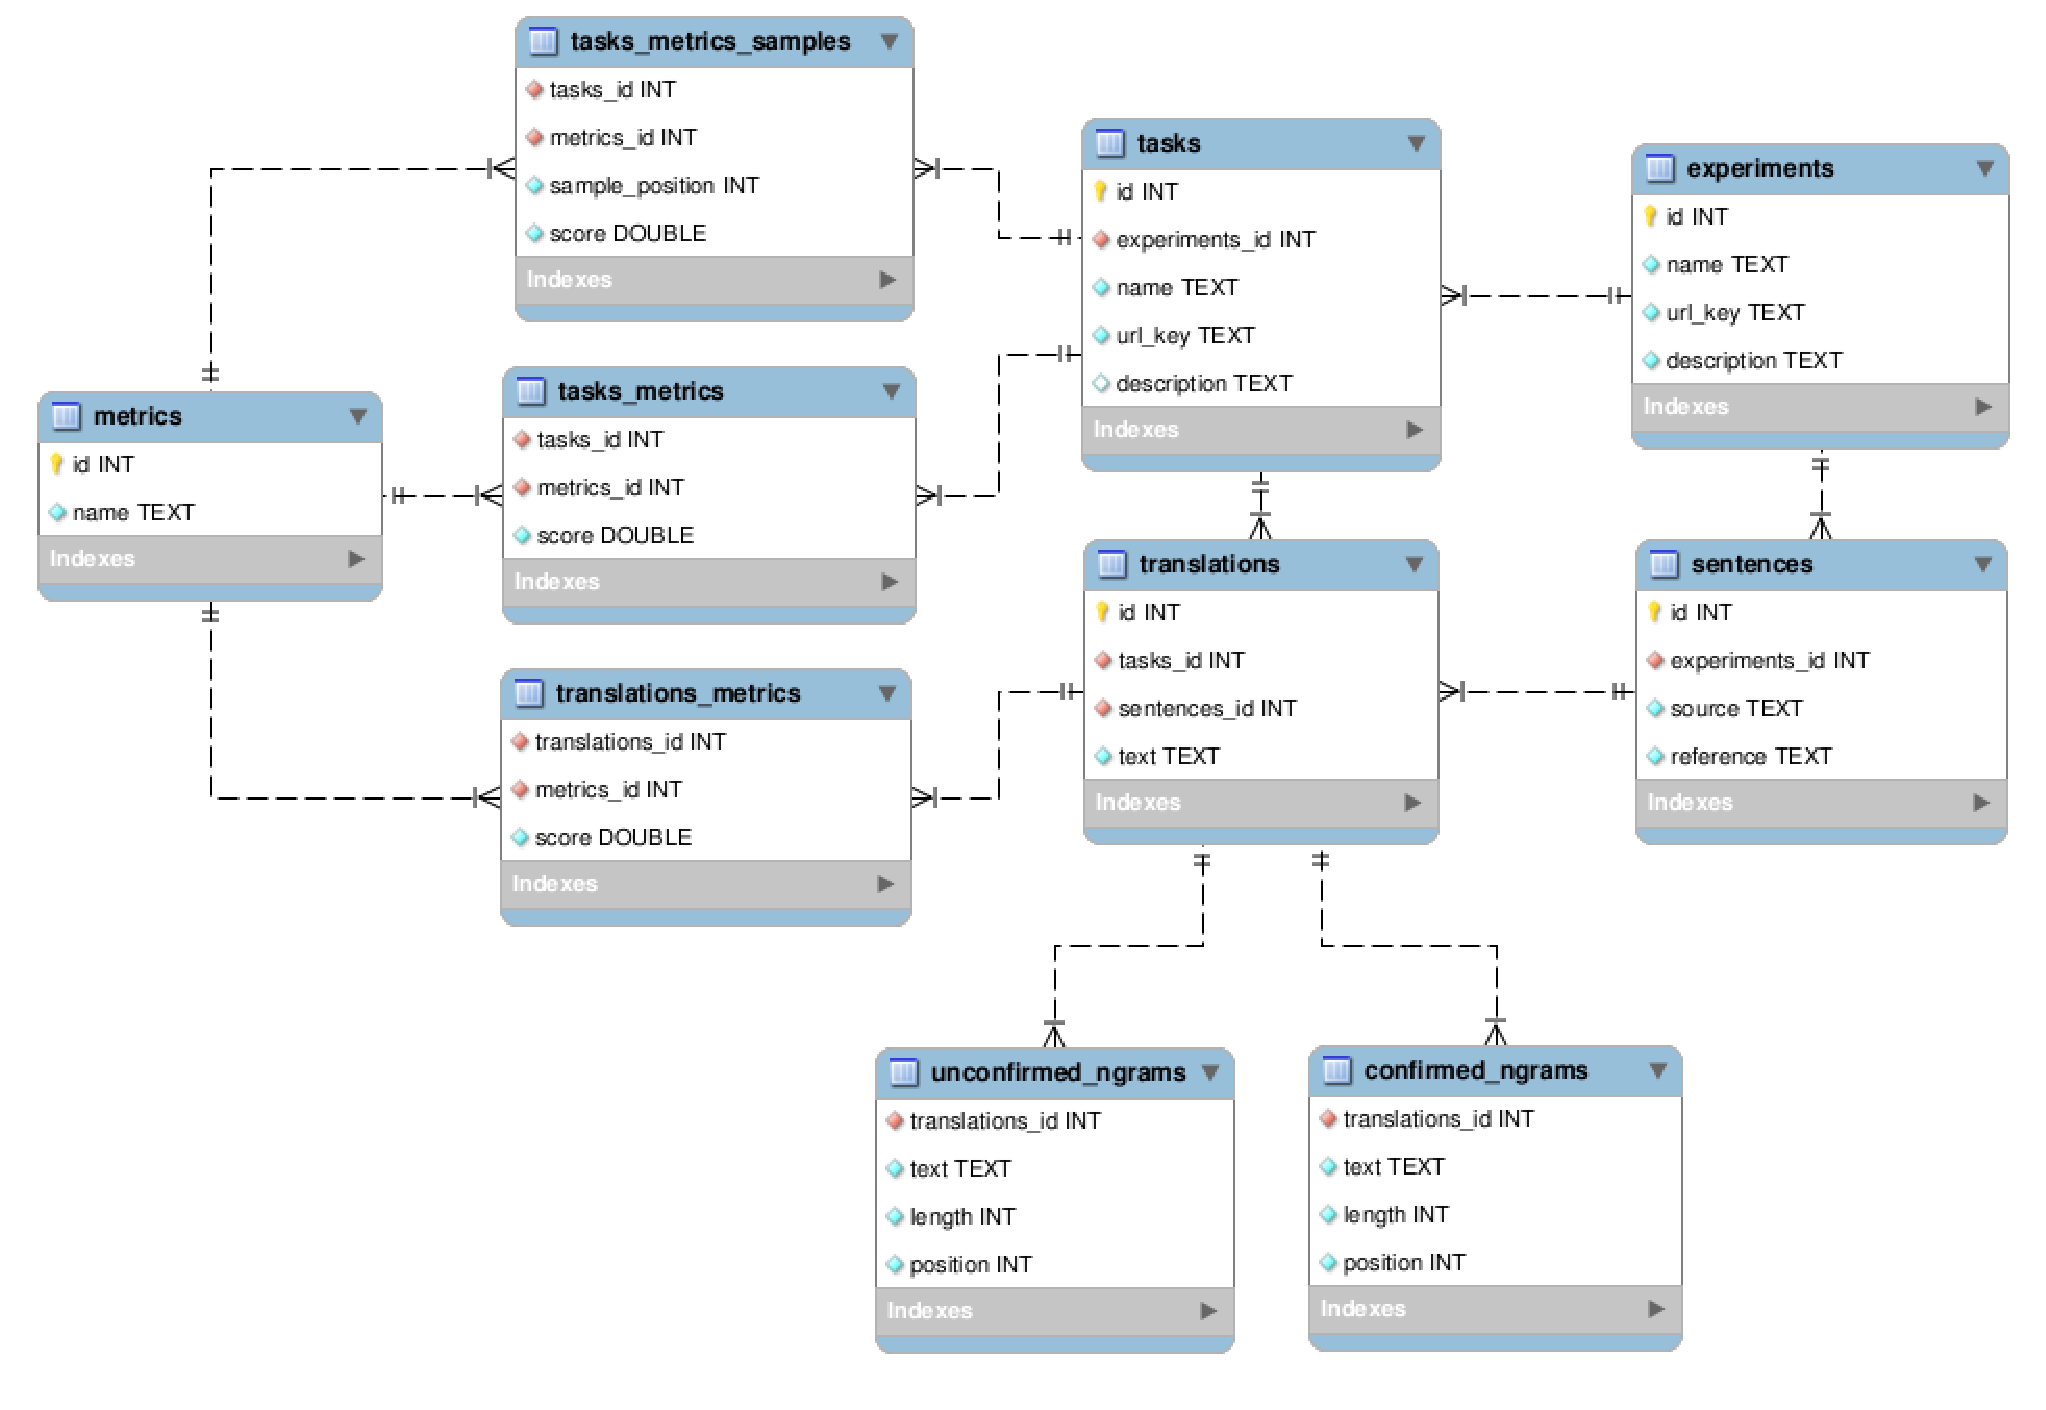
\includegraphics[width=0.8\textwidth]{img/schema.eps}}}
\section{Import experimentů a tásků}
\section{REST API}
\section{Frontend}

MT-ComparEval slouží k porovnávání a vyhodnocování strojových překladů.
Hlavním požadavkem při vývoji aplikace bylo,
  aby bylo možné jednoduše sputit aplikaci na vývojářově počítači.
Proto byly použity technologie,
  které jsou běžně dostupné na většině linuxových distribucí.
Jako hlavní programovací jazyk byl použit jazyk PHP ve verzi 5.4 
  s použitím frameworku Nette\footnote{http://www.nette.org}
  a jako databáze byla použita databáze SQLite3\footnote{http://www.sqlite.org}.
Jazyk PHP ve verzi 5.4 má v sobě obsažen jednoduchý webový server,
  tudíž je možné aplikaci bez větších obtíží spustit na vývojářově počítači.
V případě, že by měla aplikace běžet na serveru,
  je možné použít např. Apache HTTP Server.
Pokud by měla aplikace zpracovávat velké množství překladů,
  je možné použít i jiné databáze,
  ale bude potřeba přizpůsobit konfiguraci aplikace.
Na frontendu byl použit javascript s frameworkem AngularJS.\footnote{http://www.angularjs.com}


MT-ComparEval je webová aplikace skládající se ze tří částí:

\begin{itemize}
	\item serverové části pro import jednotlivých překladů
	\item serverové části pro vykreslování šablon a REST API
	\item frontendové části pro interaktivní porovnávání překladů
\end{itemize}

\section{Import překladů}
Aplikace MT-ComparEval byla navržena tak,
  aby ji bylo možné snadno zasadit do vývojového procesu strojových překladů.
Nepředpokládali jsme,
  že by si uživatel manuálně nahrával jednotlivé překlady k porovnání.
Spíše se předpokládá, že uživatel bude mít nastavený vývojový proces tak,
  že po každém úspěšném překladu se výsledný překlad nahraje do naší aplikace,
  kde si uživatel bude moci prohlédnout daný překlad v porovnání s ostatními překlady.

Vyhodnocování projektu probíhá proti referenčnímu překladu od překladatele.
Aby uživatelé mohli porovnávat své překladové systémy proti různým referenčním překladům,
  je možné si v naší aplikaci vytvořit různé uv{experimenty}. 

Experiment obsahuje zdrojový text, z kterého vznikaly překlady, a referenční překlad.
Každý experiment je uložen jako adresář,
  který obsahuje soubor se zdrojovým textem, referenčním překladem
  a konfigurační soubor.
V současné době aplikace umožňuje mít pouze jeden referenční překlad v experimentu,
  protože i ve většině soutěží se používá pouze jeden referenční překlad.

Do každého experimentu si může uživatel libovolně nahrávat nové strojové překlady.
V aplikaci tyto překlady nazývame uv{tasky}.
Každý task je uložen jako podadresář adresáře s experimentem
  a obsahuje soubor se strojovým překladem
  a konfigurační sobour. 

U všech souborů s překlady předpokládáme, že jsou zarovnané po větách.
Konfigurační soubory v obou případech slouží k přidání metainformací o experimentu/tasku,
  které mohou být později použity ve webové aplikaci.

\subsection{Import experimentů}
Všechny experimenty, které chceme naimportovat do naší aplikace,
  se musí uložit do adresáře \textbf{./data} v kořenu aplikace.
Nad tímto adresářem bdí proces, který hlídá,
  jestli zde nepřibyl nějaký nový experiment.
V případě, že objeví nějaký nový experiment,
  spustí další proces, který tento experiment naimportuje.

Při importu experimentu se nahrají všechny zdrojové věty
  a referenční překlady do databáze,
  abychom je mohli později použít při importu tasků
  nebo zobrazování výsledků.

Po úspěšném importu je do adresáře s experimentem přidán soubor,
  který nám označí daný experiment jako úspěšně naimportovaný.
Toho využijeme při importu tasků,
  abychom se nepokoušeli importovat tasky v experimentech,
  které ještě nebyly úspěšně naimportovány.
Zárověň tento zámek využijeme k tomu,
  abychom některý experiment nenaimportovali vícekrát.

%% TODO zamek pro neuspesne importy
Při importu experimentů může dojít k různým chybám -
  ať už na straně uživatele nebo na straně MT-ComparEval.
V případě, že nějaká chyba nastane,
  je do adresáře s experimentem přidán soubor,
  který nám označí,
  že při importu experimentu došlo k chybě
  a neměli bychom se ho pokoušet importovat znovu.
Když uživatel opraví chybu,
  která způsobila neúspěch importu,
  může tento soubor odstranit
  a MT-ComparEval se pokusí daný experiment znovu naimportovat.

\subsection{Import tasků}
Tasky, které chceme naimportovat do naší aplikace,
  se musí uložit do adresářů experimentů,
  ke kterým daný task patří.
Nad těmito adresáři bdí stejný proces
  jako proces pro import experimentů.
Tento proces hledá nový task ve všech již 
  naimportovaných experimentech.

Při importu tasku se nahrají všechny přeložené věty do databáze.
Zároveň musíme celý task vyhodnotit a předpočítat hodnoty,
  které později použijeme na frontendu.
Mezi tyto hodnoty patří:
\begin{itemize}
	\item metriky pro celý překlad a jednotlivé věty
	\item hodnoty pro Bootstrap Resampling 
	\item zlepšující/zhoršující n-gramy
\end{itemize}

\subsubsection{Předzpracování vět}
Jelikož se při importu tasků mnohé výpočty opakují
  ( počítání metrik, boostrap resampling, hledání společných n-gramů, \dots ),
  chceme si je předpočítat,
  abychom je mohli později použít a nemuseli je pokaždé počítat znovu.

Pokud chceme,
  aby naše výsledky výpočtu metrik byly stejné jako u jiných nástrojů,
  musíme text nejprve znormalizovat.
Znormalizování nám přidá mezery před a za všechna interpunkční znaménka.
Tím nám oddělí všechna slova a diakritiku - dále je budeme nazývat tokeny.
Znormalizovaný text můžeme tokenizovat (rozdělit na jednotlivá slova a diakritiku).
S takto získanými tokeny můžeme počítat libovolné metriky,
  aniž bychom se museli bát,
  že se naše výsledky budou lišit od výsledků jiných nástrojů.

Dalším krokem při předzpracování je získaní všech n-gramů z referenčního a strojového překladu.
N-gramem rozumíme posloupnout n po sobě jdoucích slov.
V nástroji MT-ComparEval počítáme pouze s n-gramy délky 1-4,
  tudíž při předzpracování hledáme pouze n-gramy těchto délek. 

Z n-gramů ze strojového překladu najdeme potvrzené n-gramy
  ( vyskytují se i mezi referenčními n-gramy )
  i n-gramy nepotvrzené.
Z těchto n-gramů později vypočítáme n-gramy,
  které nejvíce zlepšují/zhoršují skóre daného systému.
  
Jelikož při výpočtu BLEU nepotřebujeme znát jednotlivé n-gramy,
  z předpočítaných n-gramů si uložíme pouze jejich počty podle délky.
To nám ušetří mnoho času při výpočtu hodnot pro bootstrap resampling.

\subsubsection{Zpracování vět}
Hlavním cílem při zpracování vět je spočítat metriky jak pro jednotlivé věty,
  tak pro celé překlady.
Pomocí metrik u jednotlivých vět můžeme řadit věty tak,
  abychom zobrazili pouze věty, 
  které nás zajímají.
To jsou věty, u kterých došlo k největší změně.
%% vlozit screenshot s ukazkami vet
Pomocí metrik u celých překladů můžeme rozhodnout,
  který překlad je lepší
  nebo jestli se námi používaný překladový systém zlepšuje/zhoršuje.
%% vlozit ukazku vypisu tasku.

Metriky se počítají vždy v páru - case sensitive / case insensitive.
To proto, že se potvrzený n-gram může nacházet v referenčním překladu na začátku věty,
  kde bude začínat velkým písmenem,
  ale ve strojovém překladu se bude nacházet uprostřed věty,
  kde bude začínat malým písmenem.
%% vlozit ukazku vety, ktera zacina potvrzeným n-gramem.
Potom budou dávat obě metriky různé výsledky 
  a je jen na uživateli,
  aby si zvolil, která metrika ho více zajímá.

Aby si uživatel mohl doimplementovat další metriky,
  může TaskImporter použít libovolné množství implemantací rozhrani Metric.
Díky tomu je možné porovnávat výsledky pomocí různých metrik.

\subsubsection{Dokončení importu}
Před tím, než nahrajeme data do databáze, je nutné,
  abychom si dopočítali poslední informace,
  které potřebujeme ke správnému chodu frontendu,
  ale které jsou výpočetně náročné,
  tudíž by trvalo dlouhou dobu,
  než by je REST API spočítalo.

Mezi tyto informace patří vygenerovaní vzorků pro bootstrap resampling a
  nalezení nejvíce zlepšujících resp. nejvíce zhoršujících n-gramů.

\subsubsection{Bootstrap resampling}
%% rozsirit sekci o bootstrap resamplingu
Abychom mohli efektivně porovnávat dva překlady pomocí metody bootstrap resampling,
  musíme si předgenerovat velké množství náhodných vzorků.
My chceme,
  abychom vždy porovnávali stejné vzorky,
  ale abychom je nemuseli počítat při každém porovnávání počítat znovu.
Na začátku generování náhodných vzorků tedy nastavíme stejné jadérko generátoru náhodných čísel.
Tím dosáhneme toho,
  že všechny vzorky budou obsahovat vždy stejné věty
  a nemusíme tedy generovat vzorky pro všechny dvojice tasků v experimentu.
Náhodné vzorky počítáme pro všechny dostupné metriky,
  protože rozhraní pro výpočet jednotlivých metrik nám umožňuje spočítat danou metriku pro libovolnou testovací sadu,
  můžeme tyto výpočty znovu použít.


\subsubsection{Hledání nejvíce zlepšujících/zhoršujících n-gramů}
Nástroj MT-ComparEval nabízí i výpis nejvíce zlepšujících resp. nejvíce zhoršujících n-gramů.
Ty získáme tak, že vezmeme všechny potvrzené resp. nepotvrzené n-gramy
  a uděláme rozdíl obou porovnávaných překladů.
N-gramy,
  které mají největší rozdíl mezi jednotlivými překlady,
  jsou nejvíce zlepšující resp. nejvíce zhoršující.

Jelikož potvrzených resp. nepotvrzených n-gramů může být velké množství
  a nalezení nejvíce zlepšujících resp. nejvíce zhoršujících n-gramů může být pomalé,
  je potřeba,
  abychom našli všechny zlepšující resp. zhoršující n-gramy předem.
Při importu tasku tedy vezmeme všechny ostatní tasky z daného experimentu
  a pro ně předpočítáme 10 nejvíce zlepšujících resp. zhoršujících n-gramů. 

Abychom udělali počítání zlepšujících resp. zhoršujících n-gramů co nejefektivnější,
  používáme algoritmus podobný mergesortu,
  který z databáze postupně načítá n-gramy seřazené podle textu a věty, ve které se nacházejí, 
  a slévá je dohromady tak, že:

\begin{itemize}
  \item Pokud jsou oba n-gramy stejné, můžeme pokračovat ve výpočtu s další dvojicí.
    Pouze zaktualizujeme počet výskytů n-gramů v jednotlivých překladech. 
  \item Pokud se n-gramy liší, přidáme zlepšující resp. zhoršující n-gram k překladu,
    ve kterém se nachází uv{menší n-gram}. \\
    uv{Menší n-gram} je ten, který se nachází ve větě s nižším pořadovým číslem
    nebo je lexikograficky menší.
\end{itemize}

Na závěr vybereme 10 nejlepších resp. nejhorších n-gramů
  a uložíme si je pro pozdější použití.
Tímto alogirtmem dosáhneme lineární paměťové složitosti a
  lineární časové složitosti v závislosti na počtu potvrzených resp. nepotvrzených n-gramů.

%% TODO dodelat vypnuti predpocitani tasku
I přes to, že časová složitost předpočítání je lineární,
  může být předpočítání pro všechny ostatní tasky časově náročné
  (časová složitost je lineárně závislá na počtu tasků v experimentu),
  proto je možné toto předpočítání v konfiguraci jednotlivých tasků vypnout.
V porovnání dvou tasků pak nebudou předpočítané n-gramy k dispozici
  a je potřeba spustit skript,
  který je pro daný task zpětně dopočítá.

\subsubsection{Uložení předpočítaných dat do databáze}
Předpočítaná data pro jednotlivé tasky ukládáme do databáze SQLite3.
Při importu tasků chceme uložit velké množství dat,
  což by mohlo trvat velmi dlouho.
Proto jsou všechna data uložena v jedné transakci,
  která je mnohem rychlejší,
  než postupné ukládání.
Navíc tím získáme jistotu,
  že se nám do databáze nedostanou tasky,
  jejichž import se z různých důvodů nemusel povést.
 
\subsubsection{Logování importů}
%% přidat ukázky logů
Všechny důležité operace spojené s importem tasků či experimentů
  ( ať už je to načítání konfiguračního souboru, načítání vět ze souborů,
  počítání metrik, ukládání do databáze nebo některé další ), 
  jsou logovány do souboru,
  z kterého později můžeme vyčíst,
  proč nebyl některý task či experiment úspěšně naimportován. 


\section{REST API}
REST API je implementované v jazyce PHP s použitím frameworku Nette.
Slouží k předávání předpočítaných informací frontendu,
  který si je dle potřeby získává za použití AJAXu.
Api vždy vrací data ve formátu JSON,
  který můžeme snadno použít v javascriptu.
Pomocí api navíc můžeme získávat pouze data,
  která v danou chvíli potřebujeme.
Tzn. že nebudeme načítat všechny věty naráz,
  ale můžeme si je načítat postupně,
  s tím jak si je uživatel prohlíží.
Stejně tak nemusíme stahovat všechna data pro grafy,
  ale stačí nám stáhnout data pro právě vybranou metriku.

Pomocí api získáváme většinu dat pro porovnání dvou překladů,
  ať už jsou to dostupné metriky,
  data pro vykreslení grafů právě vybrané metriky,
  zlepšující resp. zhoršující n-gramy
  nebo věty,
  které můžeme řadit podle libovolné metriky a získavat je po částech.

V případě, že bychom chtěli zefektivnit použítí api tak,
  aby se všechna data musela počítat pouze jednou,
  můžeme použít reverse proxy cache - např. Varnish Cache.
To nám může výrazně ušetřit výpočetní výkon a zlepšit dobu odezvy api v případě,
  že aplikaci bude používat hodně uživatelů
  a bude v ní nahráno hodně experimentů/tasků.

\section{Frontend}
Na frontendu byl použit CSS framework Bootstrap od firmy Twitter,
  díky kterému bylo jednoduché vytvořit poměrně působivý design,
  a javascriptový framework AngularJS.
Jedná se o MVC framework vyvíjený ve firmě Google,
  mezi jehož hlavní přednosti patří 2-way data binding -
  tzn. že při změně v modelu nebo nějaké uživatelské interakci se stránky automaticky překreslí.
Díky tomu je možné deklarativně popsat chování stránek,
  které pak si při každé uživatelské akci stáhnou potřebná data z api
  a není tak potřeba psát kód pro různé situace.

Na frontendu se nacházejí tři typy stránek:
\begin{itemize}
  \item seznam všech experimentů
  \item seznam všech tasků v daném experimentu
  \item porovnání dvou tasků
\end{itemize}

Seznamy experimentů a tasků slouží pouze k výběru tasků,
  které chceme porovnávat,
  proto se jedná pouze o výpis jmen s upřesňujícími informacemi.

%% TODO přidat graf vývoje 
V seznamu tasků daného experimentů navíc můžeme vidět graf s vývojem jednotlivých metrik tasků.
Pomocí něho si můžeme rychle udělat přehled,
  jak se překlady zlepšují resp. zhoršují.
Pokud by nám informace z grafu nestačily,
  je možné najít přesné hodnoty metrik v tabulkách u jednotlivých tasků.
Na základě těchto informací si můžeme vybrat,
  které tasky má smysl porovnávat.
Díky jednoduchému procházení experimentů a tasku se můžeme zaměřit na nejdůležitější část aplikace
  - porovnávání dvou tasků.

Dva tasky můžeme porovnávat na základě několika kritérií,
  kterým odpovídá záložka na stránce s porovnáním dvou tasků:
%% TODO přidat obrázek s výběrem záložek
\begin{itemize}
  \item Sentences - porovnání na základě překladu jednotlivých vět
  \item Statistics - porovnání na základě výsledků jednotlivých metrik
  \item Confirmed n-grams - porovnání na základě nejvíce zlepšujících n-gramů
  \item Unconfirmed n-grams - porovnání na základě nejvíce zhoršujících n-gramů
\end{itemize}

Abychom nemuseli složitě přecházet mezi stránkami,
  když chceme porovnávat jiné tasky z experimentu,
  je možné měnit tasky přímo v porovnání.


\subsubsection{Porovnání na základě překladu jednotlivých vět}
Při porovnávání dvou překladů nás nejvíce zajímají věty,
  které se nejvíce zlepšily resp. zhoršily.
To poznáme tak, že se rozdíl metrik nejvíce liší. 
Proto jsou věty vždy seřazeny podle rozdílů metrik.
Metriky můžeme libovolně měnit a stránka se automaticky zaktualizuje.
Zároveň se změnou metriky můžeme ovlivnit,
  v jakém pořadí budou věty načítány.
Tím můžeme určit,
  jestli nás zajímají věty,
  které se nejvíce zlepšily resp. zhoršily.
Jelikož načtení všech vět by mohlo být náročné,
  načítají se vždy věty s tím,
  jak se uživatel postupně posouvá stránkou.
Často nám stačí prohlédnout pouze několik vět,
  abychom si udělali obrázek,
  v čem se dva porovnávané tasky nejvíce liší.
Aby si mohl uživatel vybrat,
  které překlady ho zajímají,
  může si skrýt a zobrazit zdrojovou větu, referenční překlad nebo porovnávané překlady.
Toho může využít, když ho zajímá např. pouze porovnání jednoho překladu s referencí a
  ostátní překlady by ho mohly rušit.

%% vložit obrázky s porovnáváním vět a zvýrazněnými potvrzenými, zlepšujícími nebo zhoršujícími n-gramy
Aby uživatel mohl snáz porovnávat překlady vět,
  může si dle chuti zapnout / vypnout zvýraznění všech potvrzených n-gramů,
  zlepšujících n-gramů nebo zhoršujících n-gramů.
Za zlepšující n-gramy jsou považovány ty potvrzené n-gramy,
  které se nacházejí pouze v jednom z porovnávaných překladů.
To stejné platí pro zhoršující n-gramy,
  které ale vybíráme z nepotvrzených n-gramů.
Na základě barevného podbarvení jednotlivých slov pak uživatel může poznat,
  která slova jsou přeložena lépe či hůře.

Další možností jak rychle porovnat překlady je zvýraznit diff mezi překladem a referenčním překladem.
Ve většině případů se toto zvýraznění nebude odlišovat od zvýraznění potvrzených n-gramů -
  zvýrazněné potvrzené n-gramy se nacházejí jak v referenčním tak v porovnávaném překladu
  a nezvýrazněná slova se nenacházejí v jednom z překladů.
Jediný rozdíl mezi těmito zvýrazněními nastane,
  když se bude lišit slovosled porovnávaných překladů,
  pak může být povrzený n-gram označen za chybějicí resp. přebývající.

\subsubsection{Porovnání na základě výsledků jednotlivých metrik}
%% vlozit obrazek s porovnáním vysledku dvou tasku
Rychlý přehled o kvalitě jednotlivých překladů si můžeme udělat pohledem na výsledky jednotlivých metrik.
Ať už se jedná o data v tabulce s metrikami nebo graf hodnot jednotlivých metrik,
  graf rozdílů aktuální metriky u vět nebo graf bootstrap resamplingu.
Grafy se automaticky překreslují při změně metriky,
  podle které se mají řadit věty,
  tím si může uživatel zobrazit grafy pro všechny nabízené metriky.


\subsubsection{Porovnání na základě nejvíce zlepšujících resp. zhoršujících n-gramů}
%% vlozit obrázek s výpisem nejvíce zlepšujících / zhoršujících n-gramů
Dobrý obrázek o zlepšení / zhoršení překladu si můžeme udělat,
  když se podíváme,
  v kterých n-gramech se dané překlady nejvíce liší,
  ať už se jedná o zlepšující n-gramy nebo n-gramy zhoršující.
Nástroj MT-ComparEval vypisuje seznam zlepšujících resp. zhoršujících n-gramů seskupených podle délky,
  pomocí něhož můžeme filtrovat věty a prohlížet si pouze ty,
  v kterých se daný zlepšující resp. zhoršující n-gram nachází.
Vybraný n-gram je následně ve všech větách zvýrazněn,
  aby uživatel mohl rychle zjistit, kde se nachází -
  může se totiž stát, že se daný n-gram ve větě bude nacházet vícekrát,
  ale pouze některý z nich bude zlepšující resp. zhoršující.

Jelikož se daný n-gram může nacházet v mnoha větách,
  nenačítáme všechny věty naráz,
  ale věty jsou načítány postupně,
  stejně jako když procházíme věty v normálním režimu.
Stejně tak se může stát,
  že se v jedné větě vyskytne zlepšující n-gram vícekrát
  ( typicky se to stává u interpunkce, spojek nebo předložek ),
  tyto věty nás zajímají více než věty,
  ve kterých je výskytů daného n-gramu méně.
Proto jsou věty při filtrování podle zlepšujícího resp. zhoršujícího n-gramu vždy řazeny podle počtu výskytů daného n-gramu ve větě
  a nejde je řadit podle rozdílu metrik jako v normálním módu.

%% vlozit obrazek zhorsujiciho n-gramu, ktery obsahuje zlepsujici n-gram
Při zobrazování delších zhoršujících n-gramů může nastat situace,
  že si uživatel nechá zvýraznit všechny zhoršující n-gramy,
  ale vybraný zhoršující n-gram nebude zvýrazněn.
Dokonce se může stát, 
  že si uživatel nechá zvýraznit všechny potvrzené n-gramy
  a část vybraného zhoršujícího n-gramu bude zvýrazněna.
Toto je úplně normální jev,
  který je způsoben výběrem potvrzených n-gramů,
  je jedno, kde se daný potvrzený n-gram nachází,
  stačí,
  že se někde ve větě objeví a už je prohlášen za potvrzený.
Změnou slovosledu pak může dojít i k situaci,
  kdy se zhoršující n-gram velké délky bude skládat z potvrzených n-gramů délky kratší,
  které se nacházely na různých pozicích ve větě. 
Například stačí, aby byly ve správném pořadí,
  ale bylo mezi nimi vypuštěno alespoň jedno slovo.
Proto je lepší,
  aby uživatel porovnával překlady spíše podle n-gramů s menší délkou -
  typicky podle 1-gramů a 2-gramů.
Aby mělo smysl porovnávat překlady podle delších n-gramů,
  musel by být překladač otestován na velké počtu vět tak,
  aby se zlepšení resp. zhoršení dostatečně projevilo.

\section{Zobrazení potvrzených n-gramů a diffu pomocí}
Pro správné zobrazení potvrzených n-gramů a diffu je potřeba,
  abychom mohli každému tokenu říci,
  jestli se nachází v nějakém potvrzeném n-gramu nebo jestli byl do věty přidán.
Zároveň s touto informací chceme,
  aby jednotlivá zvýraznění bylo možné libovolně kombinovat.
Technicky tento problém byl vyřešen pomoci CSS tříd,
  kdy každému tokenu byly přiřazeny třídy v závislosti na informacích,
  které jsme si vypočítali pomocí výše uvedených postupů.
Zapnutí a vypnutí jednotlivých kombinací je pak otázkou přiřazení příslušné třídy kořenovému elementu,
  v kterém se nacházejí všechny věty.
Přehlednost těchto kombinací nemusí být vždy zcela ideální, 
  proto jsme se snažili udělat jednotlivá zvýraznění tak,
  aby byla co nejjednodušeji modifikovatelná.
Každý typ zvýraznění tak má vlastní selektor,
  pomocí kterého může zvýraznění v CSS upravit.



\chapter{Závěr}

\section{Současný stav aplikace}
Nástroj MT-ComparEval je v současné době plně funkční.
Umožňuje spravovat experimenty a jejich tasky.
Tasky je možné porovnávat na základě různých kriterií -
  hodnot metrik strojového překladu,
  porovnání jednotlivých vět
  či přehledu nejvíce zlepšujících a zhoršujících n-gramů.
Při porovnání překladů jedné věty je možné si nechat zvýraznit
  potvrzené n-gramy, zlepšující n-gramy, zhoršující n-gramy, diff mezi překlady
  či jeden z nejvíce zlepšujících nebo zhoršujících n-gramů.


\section{Nápady na vylepšení}
I přes to, že nástroj MT-ComparEval umožňuje porovnávat dvě různé verze překladů,
  existuje mnoho způsobů,
  jak by tento nástroj šlo vylepšit.

\subsection{Podpora více referencí}
Při vyhodnocování strojových překladů a počítání metrik používá nástroj MT-ComparEval pouze porovnání s jednou referencí.
Protože většina vět může být přeložena různými způsoby,
  může nastat situace,
  kdy daný překlad neodpovídá zvolené referenci.
Aby bylo možné takové překlady lépe ohodnotit,
  mohly by být překlady porovnávány s několika různými referencemi.
Z těchto referencí by pak byla vybrána ta,
  pro kterou by daný překlad dosáhl nejlepšího skóre.
Z tohoto důvodu by bylo dalším možným rozšířením přidání podpory více referencí v experimentu.

\subsection{Více metrik}
I přes to, že metrika BLEU silně odpovídá lidskému hodnocení překladů,
  nemusí být vždy považována za nejvhodnější pro jejich vyhodnocování.
Některé strojové překladače jsou speciálně optimalizovány na metriku BLEU,
  což ale v konečném výsledku nemusí dávat zcela vhodné překlady.
Proto by bylo dalším vhodným rozšířením,
  vyhodnocování strojových překladačů na základě několika metrik.
Mezi metriky,
  které by bylo možné a vhodné do nástroje MT-ComparEval doprogramovat,
  patří např. NIST, METEOR, PORT,~\dots

\subsection{Zobrazení alignmentu}
Při porovnávání dvou překladů jedné věty je velmi užitečná funkce pro zvýraznění slov (nazývaná alignment),
  které odpovídají danému slovu v referenci či dalším strojovém překladu.
Díky této funkci je pak snadnější analyzovat chovaní strojových překladačů.

Na Obrázku \ref{img:alignment} je ukázáno, jak zvýrazňuje aligment překladač Google Translate.
\begin{figure}
	\center
	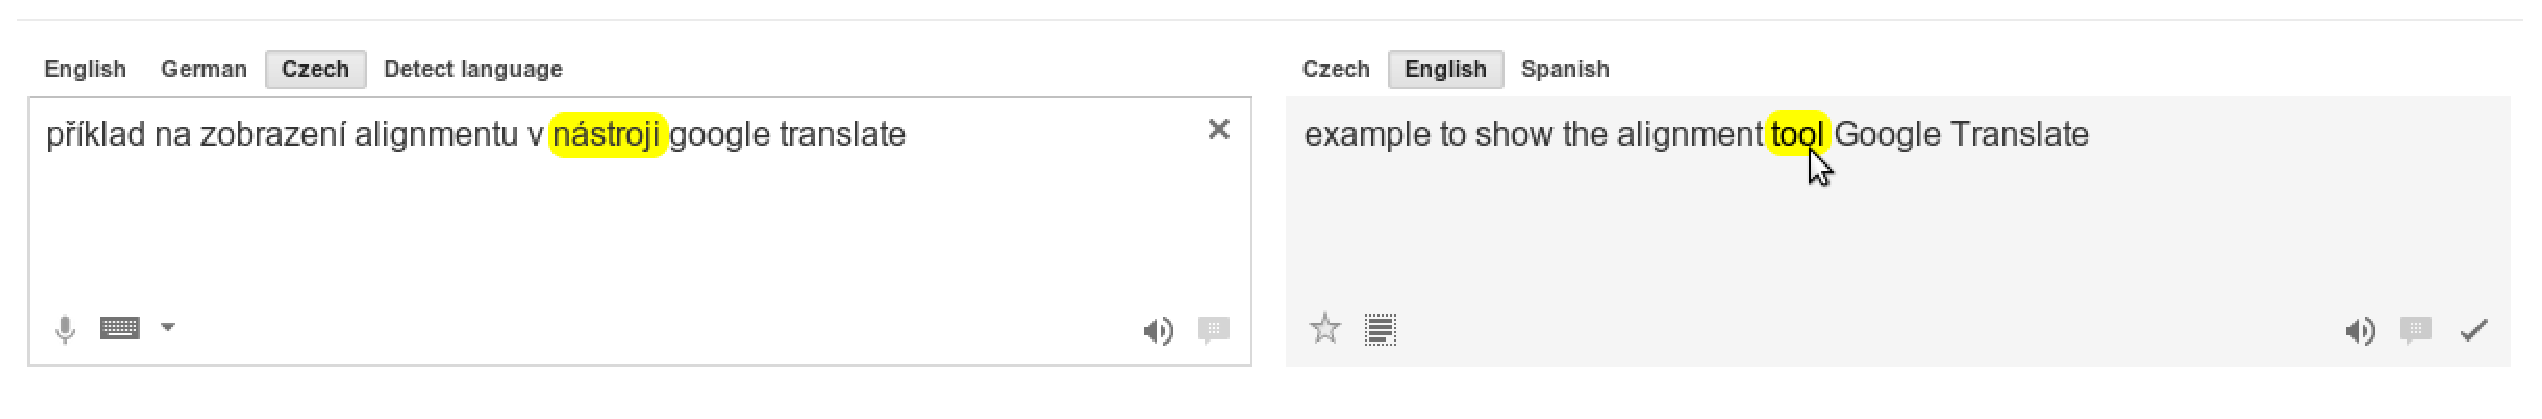
\includegraphics[width=0.9\textwidth]{img/alignment.eps}
	\caption{Ukázka zobrazení aligmentu v překladači Google Translate}
	\label{img:alignment}
\end{figure}

\section{Podobné aplikace}
Vývoj nástroje MT-ComparEval byl v určitých oblastech inspirován nástroji,
  které už jsou volně dostupné.
Z těchto nástrojů byly vybrány nejdůležitější vlastnosti,
  které byly sloučeny do jednoho funkčního celku.
V následující části budou tyto nástroje podrobněji představeny.

\subsection{mteval-11b.pl}
Je skript napsaný v jazyce Perl,
  který umožňuje počítat metriky BLEU a NIST.
Tento skript je celosvětově používaný,
  a proto byl použit pro kontrolu,
  že je metrika BLEU v MT-ComparEval počítána správně.

V současné době už existuje verze mteval-13a.pl,
  v které mimo jiné přibyla možnost počítat metriky pro jednotlivé segmenty v překladu.

\subsection{iBLEU}
Nástroj iBLEU umožňuje vyhodnocovat a porovnávat strojové překlady.
Pokud uživatel nemá žadný jiný strojový překlad,
  se kterým by chtěl svůj překlad porovnat,
  může si větu nechat přeložit překladačem Google Translate\footnote{
    Bohužel Google Translate nenabízí bezplatné api.
  } nebo Bing Translator\footnote{
    Bing Translator nabízí bezplatné api do limitu 2 miliónů přeložených znaků za den.
  }
  a porovnat svůj překlad s překladem z těchto nástrojů.

Pomocí tohoto nástroje můžeme počítat BLEU pro celé dokumenty nebo i jednotlivé segmenty.
Je také možné si jednotlivé segmenty na základě těchto výsledků prohléhnout.

Pokud uživatel porovnává svůj překlad pouze s referencí,
  je zvýrazněn jejich diff.
V případě, že uživatel porovnává dva strojové překlady,
  je zobrazen diff těchto překladů.

Tento nástroj je možné používat lokálně jako webovou aplikaci bez použití webového serveru,
  protože je celý napsán v HTML 5, CSS a javascriptu.
Stejně jako MT-ComparEval i iBLEU používá pro počítání BLEU jako referenční implementaci mteval-13a.pl.

Na Obrázku \ref{img:ibleu} je možné vidět porování dvou překladů v nástroji iBLEU.
\begin{figure}
  \center
  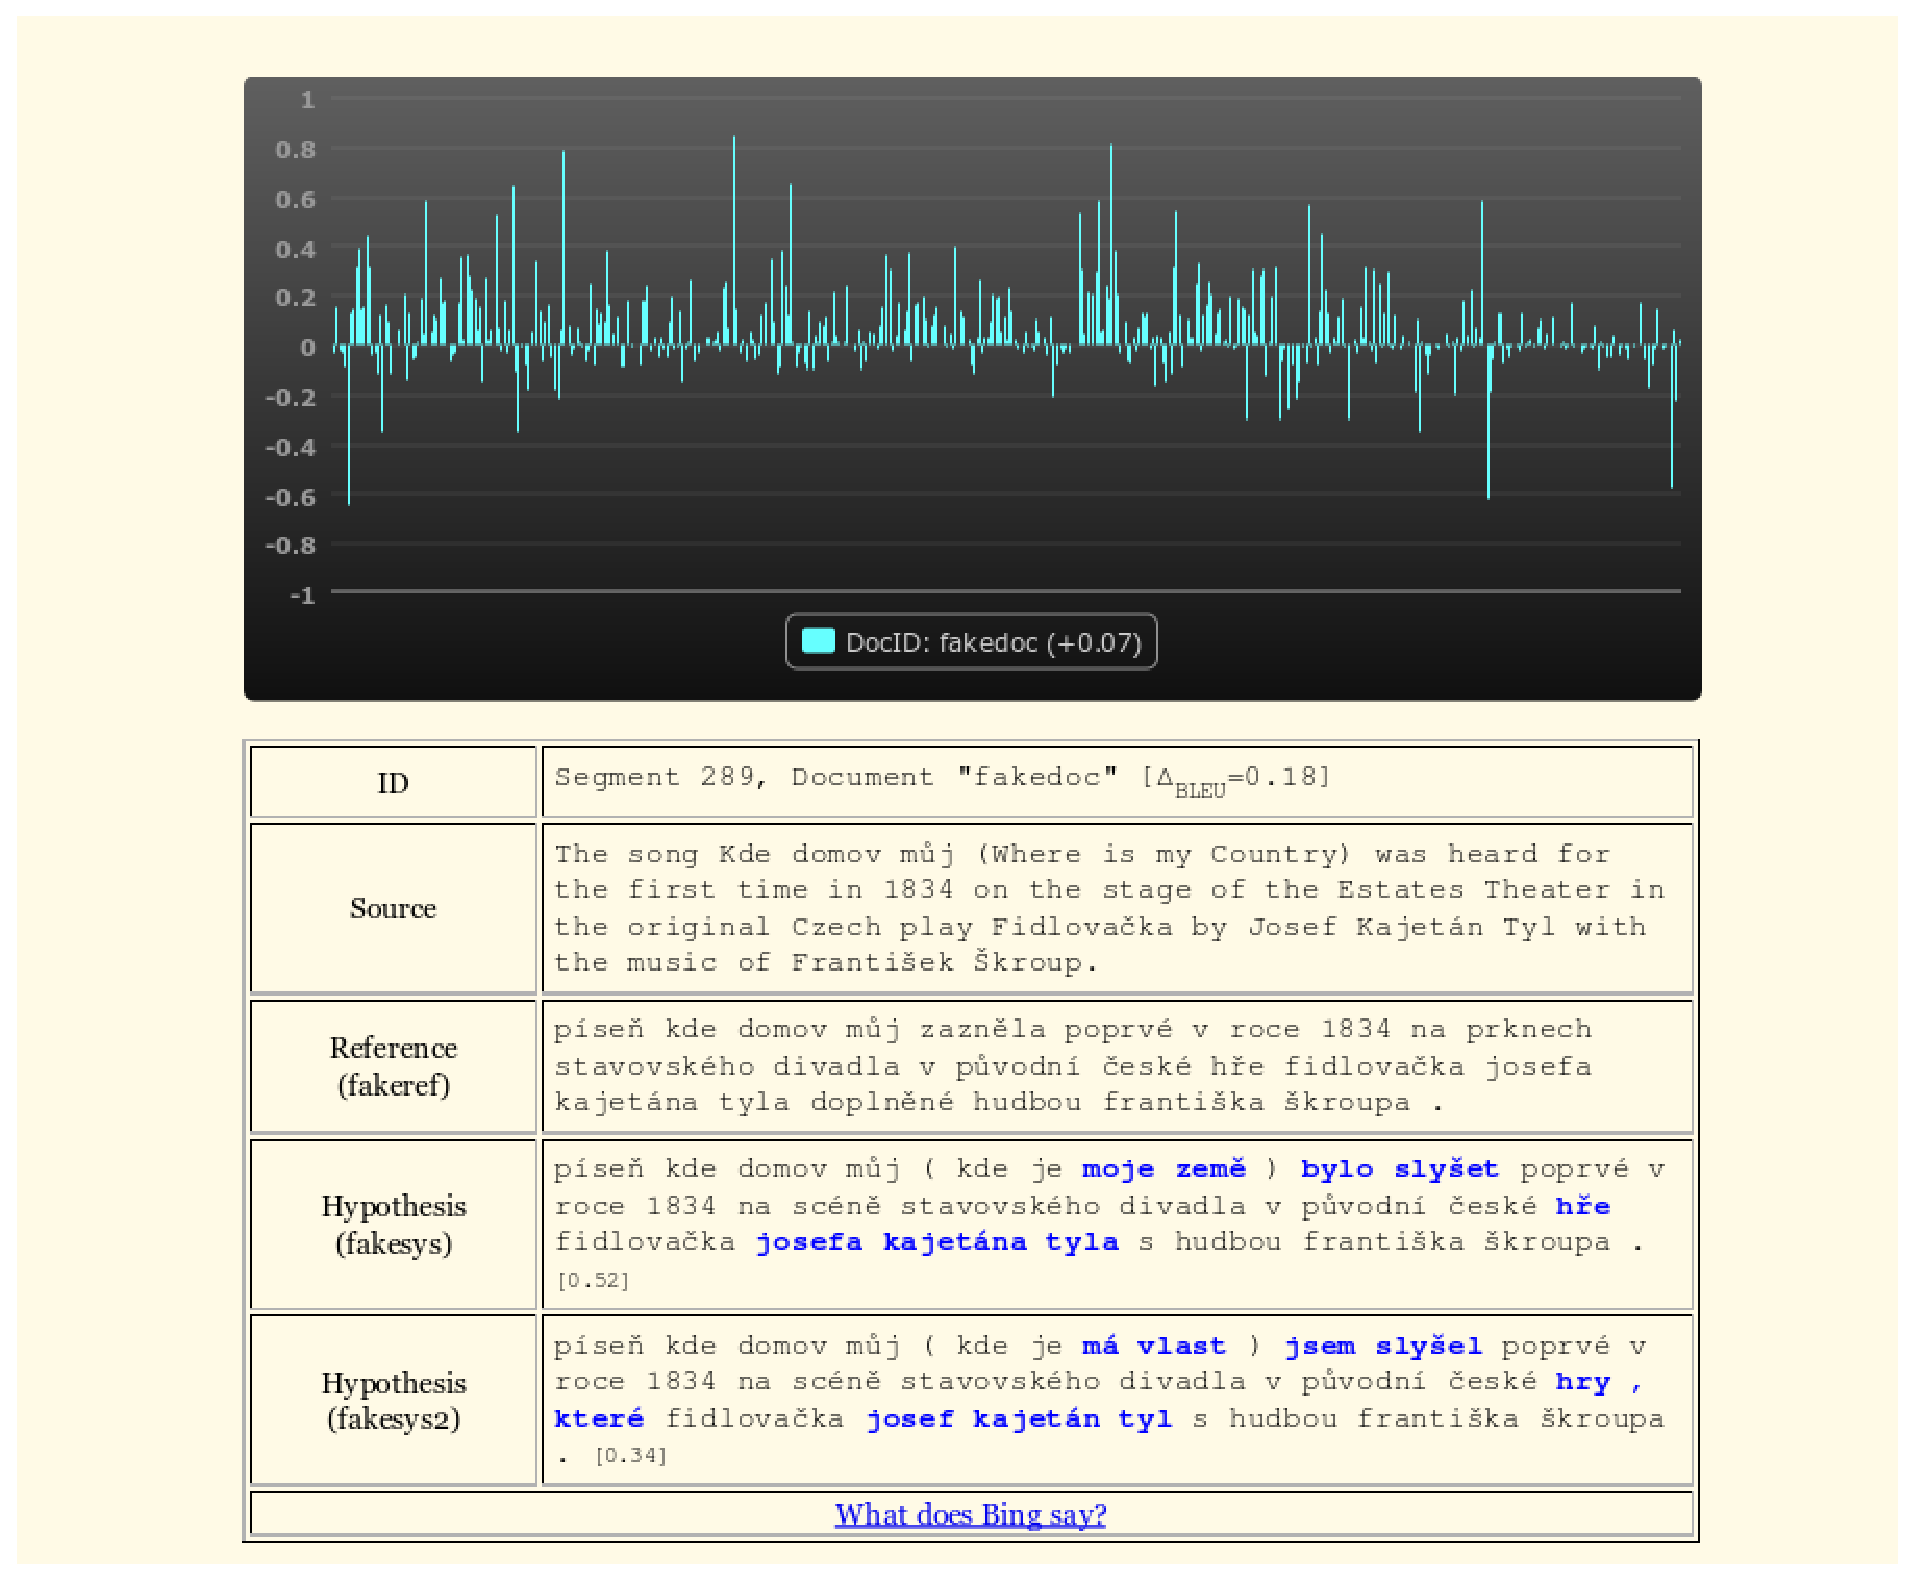
\includegraphics[width=0.9\textwidth]{img/ibleu.eps}
  \caption{Porovnání dvou překladů v nástroji iBLEU}
  \label{img:ibleu}
\end{figure}


\subsection{EMS - An Experimental Management System}
Nástroj EMS,
  který je součástí strojového překladače Moses,
  obsahuje webovou aplikaci,
  díky níž je možné porovnávat překlady.
V porovnávaných větách barevně zvýrazňuje slova,
  na základě délky nejdelšího n-gramu,
  do kterého zvýrazňované slovo patří.
Obrázek \ref{img:ems-sentence} ukazuje takto zvýrazněnou větu.
Pro n-gramy také počítá precision a recall.

\begin{figure}
  \caption{Zvýrazněné n-gramy podle délky v nástroji EMS}
  \label{img:ems-sentence}
\end{figure}

Ve webovém prostředí je také možné vyhledávat věty,
  ve kterých byl použit n-gram.
Jednotlivá užití n-gramů jsou pak rozřazena do skupin podle správnosti překladu.
Na Obrázku \ref{img:ems-word} je možné vidět seznam vět,
  ve kterých bylo použito slovo ??.

\begin{figure}
  \caption{Výpis vět, ve kterých se vyskytuje slovo ??, v nástroji EMS}
  \label{img:ems-word}
\end{figure}

Další věcí, kterou můžeme použít při porovnávání dvou překladů,
  jsou grafy správně přeložených vs. špatně přeložených slov.
Takové grafy je možné vidět na Obrázku \ref{img:ems-charts}.

\begin{figure}
  \caption{Grafy správně přeložených vs. špatně přeložených slov v nástroji EMS}
  \label{img:ems-charts}
\end{figure}

Webové prostředí nástroje EMS nabízí i další možnosti porovnání překladů,
  o kterých je možné se více dozvědět v dokumentaci tohoto nástroje.

\section{Problémy při řešení}
Při vývoji nástroje MT-ComparEval jsem narazil na mnoho problémů.
Ať už se jednalo o volbu jazyka, frameworku či databáze.

Aby bylo možné snadno nainstalovat nástroj MT-ComparEval na vybraném počítači,
  byla jako databáze zvolena databáze SQLite 3.
Ta vyhovuje většině požadavků.
Bohužel bylo hodně času věnováno odhalování chyb,
  způsobených tím,
  že SQLite 3 zamyká zvláštním způsobem datový soubor,
  a proto není možné používat databázi v dalších procesech.
Při normálním použití na webu se s touto chybou nepotkáme,
  protože procesy databázi používají pouze během zpracování HTTP požadavku.
Avšak při použití dlouho trvajících procesů pro import experimentů a tasků
  vždy docházelo ke kolizím při přístupu k databázi,
  které vyústily v pád importu.
Proto musel být návrh importu zcela přepracován a nyní by měl fungovat podle představ.
Nyní už import funguje správně a neměl by při něm nastat výše zmíněný problém.


V duchu TDD\footnote{Test-Driven-Development}
  jsem se snažil před vlastní implementací napsat testy pomocí nástroje Behat.\footnote{http://www.behat.org}
Ten slouží k BDD\footnote{Behaviour-Driven-Development}.
Pro všechny kroky importů byly napsány specifikace chování, které byly nástrojem Behat otestovány.
Ovšem později se ukázalo, že tento přístup k testování nebyl úplně vhodný, a testy pomocí tohoto nástroje jsem přestal psát.
Vše bylo způsobeno tím, že byla porušena pyramida testů\footnote{http://martinfowler.com/bliki/TestPyramid.html},
  jelikož všechny testy odpovídaly pouze funkčním testům.
Lepším řešením by bylo vytvořit pro všechny funkční požadavky unit testy,
  jejichž spuštění by trvalo kratší dobu.


%%% Seznam použité literatury
%%% Seznam použité literatury je zpracován podle platných standardů. Povinnou citační
%%% normou pro bakalářskou práci je ISO 690. Jména časopisů lze uvádět zkráceně, ale jen
%%% v kodifikované podobě. Všechny použité zdroje a prameny musí být řádně citovány.

\def\bibname{Seznam použité literatury}
\begin{thebibliography}{99}
\addcontentsline{toc}{chapter}{\bibname}

%\bibitem{lamport94}
%  {\sc Lamport,} Leslie.
%  \emph{\LaTeX: A Document Preparation System}.
%  2. vydání.
%  Massachusetts: Addison Wesley, 1994.
%  ISBN 0-201-52983-1.

\end{thebibliography}


%%% Tabulky v bakalářské práci, existují-li.
\chapwithtoc{Seznam tabulek}

%%% Použité zkratky v bakalářské práci, existují-li, včetně jejich vysvětlení.
\chapwithtoc{Seznam použitých zkratek}

%%% Přílohy k bakalářské práci, existují-li (různé dodatky jako výpisy programů,
%%% diagramy apod.). Každá příloha musí být alespoň jednou odkazována z vlastního
%%% textu práce. Přílohy se číslují.
\chapwithtoc{Přílohy}

\openright
\end{document}
